% VAE vs. DDPM on CIFAR-10 -- technical report.
% Build:  tectonic main.tex      (or: latexmk -pdf main.tex)
% Figures are read from ../../results/figures/ (the repository's results folder).
\documentclass[11pt,a4paper]{article}

% ---- layout & fonts -------------------------------------------------------------------------
\usepackage[a4paper,margin=2.3cm]{geometry}
\usepackage{microtype}
\usepackage{setspace}
\setstretch{1.08}

% ---- mathematics ---------------------------------------------------------------------------
\usepackage{amsmath,amssymb,mathtools,bm}

% ---- tables, figures, algorithms ------------------------------------------------------------
\usepackage{booktabs,tabularx,multirow,array}
\usepackage{graphicx}
\graphicspath{{../../results/figures/}}
\usepackage[font=small,labelfont=bf]{caption}
\usepackage{subcaption}
\usepackage{float}
\usepackage{algorithm}
\usepackage[noend]{algpseudocode}
\usepackage{xcolor}
\usepackage{tikz}
\usetikzlibrary{positioning,arrows.meta,fit,calc,shapes.geometric,backgrounds}
\usepackage{enumitem}
\setlist{itemsep=2pt,topsep=4pt}

% ---- references -------------------------------------------------------------------------------
\usepackage[numbers,sort&compress]{natbib}
\usepackage[colorlinks=true,linkcolor=blue!50!black,citecolor=blue!50!black,urlcolor=blue!60!black]{hyperref}
\usepackage[capitalise,noabbrev]{cleveref}
\usepackage{xurl}
% unique hyperref anchors for algorithm lines (avoids duplicate-destination warnings)
\makeatletter
\providecommand{\theHALG@line}{}
\renewcommand{\theHALG@line}{\thealgorithm.\arabic{ALG@line}}
\makeatother

% ---- colours used in the diagrams -------------------------------------------------------------
\definecolor{encC}{HTML}{DCE8F7}
\definecolor{decC}{HTML}{FBE3D6}
\definecolor{midC}{HTML}{E4F1DD}
\definecolor{latC}{HTML}{FFF2CC}
\definecolor{lineC}{HTML}{3B3B3B}

% ---- notation ------------------------------------------------------------------------------------
\newcommand{\x}{\mathbf{x}}
\newcommand{\z}{\mathbf{z}}
\newcommand{\eps}{\bm{\epsilon}}
\newcommand{\mub}{\bm{\mu}}
\newcommand{\sigb}{\bm{\sigma}}
\newcommand{\I}{\mathbf{I}}
\newcommand{\N}{\mathcal{N}}
\newcommand{\E}{\mathbb{E}}
\newcommand{\KL}[2]{D_{\mathrm{KL}}\!\left(#1\,\middle\|\,#2\right)}
\newcommand{\abar}{\bar{\alpha}}
\newcommand{\btil}{\tilde{\beta}}
\newcommand{\mutil}{\tilde{\bm{\mu}}}
\newcommand{\elbo}{\mathcal{L}_{\mathrm{ELBO}}}
\newcommand{\repo}{\url{https://github.com/Eyad-Elnakib1/Generative-models-VAE-DDPM}}
\DeclareMathOperator{\GN}{GN}
\DeclareMathOperator{\SiLU}{SiLU}
\DeclareMathOperator{\Conv}{Conv}
\DeclareMathOperator{\softmax}{softmax}
\DeclareMathOperator{\Tr}{Tr}

\title{\textbf{Variational Autoencoders vs.\ Denoising Diffusion Probabilistic Models}\\[4pt]
\large Implementation from Scratch, Benchmark and Analysis on CIFAR-10}
\author{Eyad Elnakib\\[2pt]\small Code, results and logs: \repo}
\date{October 2026}

\begin{document}
\maketitle

\begin{abstract}
\noindent
We implement two foundational deep generative models from scratch in PyTorch: the Variational Autoencoder
(VAE)~\citep{kingma2014vae} and the Denoising Diffusion Probabilistic Model (DDPM)~\citep{ho2020ddpm}. We train
three models on CIFAR-10: the DDPM in its original configuration, a VAE with the paper's own one-layer MLP, and a VAE
with a convolutional network whose capacity matches the DDPM's U-Net. All three are evaluated under one protocol
covering sample quality and diversity (FID, IS, KID, precision/recall), likelihood (bits/dim), sampling cost,
thematic consistency, memorisation and a blind rating.

The DDPM reaches an FID of $6.58$, an Inception Score of $8.59$ and a test likelihood bound of $3.79$\,bits/dim. The
bound is within $0.04$\,bits/dim of the published value, after $19\%$ of the original training. The convolutional
VAE reaches an FID of $121.9$, an IS of $3.88$ and $5.83$\,bits/dim. The VAE generates images about
$1{,}700\times$ faster, because it needs one network evaluation per image instead of $1000$. With 10-step DDIM
sampling the DDPM is still $6.6\times$ better in FID than the VAE.

We trace every observed difference to one design choice. The VAE \emph{learns} an amortised encoder into a
low-dimensional latent space and decodes in a single factorised step. The DDPM \emph{fixes} its encoder to gradual
Gaussian noising and decodes through a chain of $1000$ small, learned denoising steps.
\end{abstract}

\tableofcontents
\newpage
\section{Introduction}
\label{sec:intro}

Deep generative models learn a distribution $p_\theta(\x)$ from data and can draw new samples from it. Two
families laid the foundations of modern image generation:
\begin{itemize}
  \item \textbf{Variational Autoencoders} (VAEs)~\citep{kingma2014vae} fit a latent-variable model by maximising
        a variational lower bound with an amortised inference network.
  \item \textbf{Denoising Diffusion Probabilistic Models} (DDPMs)~\citep{sohl2015deep,ho2020ddpm} learn to invert
        a fixed, gradual noising process.
\end{itemize}
Both are trained by maximising an evidence lower bound (ELBO), yet they behave very differently in practice.

This report implements both models from first principles, trains them on CIFAR-10~\citep{krizhevsky2009cifar},
and compares them quantitatively and qualitatively, with the goal of explaining the \emph{main difference}
between the two approaches.

\paragraph{Contributions.}
\begin{enumerate}
  \item \textbf{Faithful implementations from scratch} (\cref{sec:arch,sec:training}). The DDPM reproduces the
        paper's CIFAR-10 configuration exactly (35.7M-parameter U-Net); only the training length is shortened.
        The VAE follows the original method exactly and is instantiated with two networks: the paper's MLP and a
        convolutional network built from the U-Net's blocks.
  \item \textbf{A shared, validated evaluation protocol} (\cref{sec:eval}). It covers FID, IS, KID,
        precision/recall, likelihood, the speed--quality trade-off, classifier-based thematic consistency,
        memorisation and a blind rating. Before any model was evaluated, the metrics were checked to reproduce
        published reference values on real data.
  \item \textbf{A mechanistic comparison} (\cref{sec:results,sec:qualitative,sec:discussion}). It links each
        empirical difference (blur, diversity, the ``prior hole'', likelihood, sampling cost) to the structure of
        the two models.
\end{enumerate}

\paragraph{Dataset.} We use CIFAR-10~\citep{krizhevsky2009cifar}: 50,000 training and 10,000 test images of
$32\times32$ RGB pixels in 10 classes. It is the DDPM paper's main benchmark, so published numbers exist to check our
implementation against. Its classes make thematic consistency measurable, and the Inception Score is only
meaningful on ImageNet-like natural images such as these. Every training run and every speed measurement used one
NVIDIA A100-SXM4-80GB (Google Colab), so compute and timings are directly comparable.

\paragraph{Models compared.} Throughout the report we compare three models:
\begin{itemize}
  \item \textbf{VAE-MLP}: the VAE with the network of \citet{kingma2014vae}.
  \item \textbf{VAE-Conv}: the same VAE method with a convolutional network of comparable size to the DDPM. This
        is the fair counterpart to the DDPM.
  \item \textbf{DDPM}: the model of \citet{ho2020ddpm}.
\end{itemize}

\paragraph{Code and data availability.} All code, configurations, training logs, raw evaluation outputs and
figures are public at \repo. Every number in this report is produced by the scripts in that repository.

\section{Theoretical Background}
\label{sec:background}

\subsection{Latent-variable models and the evidence lower bound}
A latent-variable model introduces unobserved variables $\z$ and defines
\begin{equation}
  p_\theta(\x) = \int p_\theta(\x \mid \z)\, p(\z)\, d\z .
\end{equation}
Maximum likelihood requires $\log p_\theta(\x)$, which is intractable for neural decoders. For any distribution
$q(\z \mid \x)$, Jensen's inequality gives the \emph{evidence lower bound}
\begin{equation}
  \log p_\theta(\x) \;\ge\; \E_{q(\z\mid\x)}\!\big[\log p_\theta(\x \mid \z)\big] - \KL{q(\z\mid\x)}{p(\z)}
  \;=\; \elbo(\x),
  \label{eq:elbo}
\end{equation}
with equality when $q(\z\mid\x)$ is the true posterior $p_\theta(\z\mid\x)$. Both models in this report maximise a
bound of this form. They differ in \emph{what} the latent variables are and \emph{whether} $q$ is learned.

\subsection{Variational Autoencoder}
\label{sec:bg-vae}

\paragraph{Generative model.} A latent code $\z\in\mathbb{R}^{d_z}$ is drawn from a standard normal prior and
decoded by a neural network into a diagonal Gaussian over pixels:
\begin{equation}
  p(\z) = \N(\z; \mathbf{0}, \I), \qquad
  p_\theta(\x\mid\z) = \N\!\big(\x;\, \mub_\theta(\z),\, \operatorname{diag}\sigb^2_\theta(\z)\big).
\end{equation}

\paragraph{Inference model (encoder).} The intractable posterior is approximated by an amortised Gaussian
\begin{equation}
  q_\phi(\z\mid\x) = \N\!\big(\z;\, \mub_\phi(\x),\, \operatorname{diag}\sigb^2_\phi(\x)\big),
\end{equation}
whose parameters are predicted by an encoder network in a single forward pass.

\paragraph{Reparameterisation.} To back-propagate through the sampling of $\z$, the sample is written as a
deterministic function of $\phi$ and an independent noise variable:
\begin{equation}
  \z = \mub_\phi(\x) + \sigb_\phi(\x)\odot\eps, \qquad \eps \sim \N(\mathbf{0},\I).
\end{equation}
The expectation in \cref{eq:elbo} is estimated with a single sample ($L=1$), as in the original paper.

\paragraph{The two ELBO terms in closed form.} With $D = 3\times32\times32 = 3072$ pixel dimensions and $d_z$
latent dimensions, the reconstruction term of one sample is
\begin{equation}
  -\log p_\theta(\x\mid\z) = \frac{1}{2}\sum_{i=1}^{D}\left[\log 2\pi + \log\sigma^2_{\theta,i}(\z)
  + \frac{\big(x_i-\mu_{\theta,i}(\z)\big)^2}{\sigma^2_{\theta,i}(\z)}\right],
  \label{eq:vae-recon}
\end{equation}
and the KL divergence between two diagonal Gaussians is analytic:
\begin{equation}
  \KL{q_\phi(\z\mid\x)}{\N(\mathbf{0},\I)} = \frac{1}{2}\sum_{j=1}^{d_z}\left(\mu_{\phi,j}^2 + \sigma_{\phi,j}^2
  - \log\sigma_{\phi,j}^2 - 1\right).
  \label{eq:vae-kl}
\end{equation}
Both sums run over \emph{all} dimensions before averaging over the batch, so the KL weight is exactly $\beta=1$. A
common implementation error averages \cref{eq:vae-recon} per pixel but sums \cref{eq:vae-kl}. That silently
multiplies the KL weight by $D=3072$ and causes posterior collapse; a unit test in the repository guards against it.

\paragraph{Generation.} A new image is obtained by drawing $\z\sim\N(\mathbf{0},\I)$ and outputting
$\mub_\theta(\z)$. This takes \emph{one} decoder evaluation.

\paragraph{Discrete data and bits/dim.} Pixels are integers $k\in\{0,\dots,255\}$. To make a continuous density a
valid bound on the discrete likelihood, we use uniform dequantisation:
\begin{equation}
  x = \frac{k+u}{128} - 1, \qquad u\sim\mathcal{U}[0,1),
\end{equation}
which maps every bin to an interval of width $w=2/256$ in $[-1,1)$. Since
$P(k) = \int_{\text{bin}} p(x)\,dx \ge w \exp\E_u[\log p(x)]$, the negative ELBO $\mathcal{B}$ (in nats) of an
image converts into a bound in bits per dimension:
\begin{equation}
  \mathrm{bpd} = \frac{\mathcal{B} + D\ln 128}{D\ln 2}.
  \label{eq:bpd}
\end{equation}

\subsection{Denoising Diffusion Probabilistic Model}
\label{sec:bg-ddpm}

\begin{figure}[t]
\centering
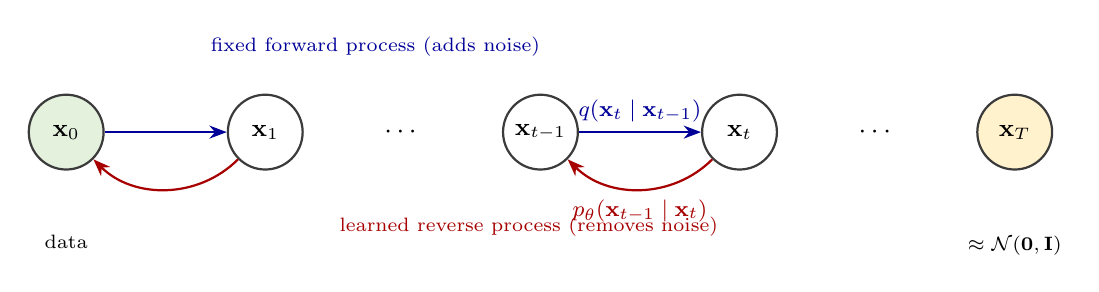
\begin{tikzpicture}[
  node distance=1.55cm,
  st/.style={circle,draw=lineC,thick,minimum size=0.95cm,inner sep=0pt,font=\small},
  fw/.style={-{Stealth[length=2.2mm]},thick,blue!60!black},
  bw/.style={-{Stealth[length=2.2mm]},thick,red!65!black},
]
\node[st,fill=midC] (x0) {$\x_0$};
\node[st,right=of x0] (x1) {$\x_1$};
\node[right=0.9cm of x1] (dots1) {$\cdots$};
\node[st,right=0.9cm of dots1] (xtm1) {$\x_{t-1}$};
\node[st,right=of xtm1] (xt) {$\x_t$};
\node[right=0.9cm of xt] (dots2) {$\cdots$};
\node[st,right=0.9cm of dots2,fill=latC] (xT) {$\x_T$};
\draw[fw] (x0) -- (x1);
\draw[fw] (xtm1) -- node[above,font=\footnotesize]{$q(\x_t\mid\x_{t-1})$} (xt);
\draw[bw] (xt) to[bend left=45] node[below,font=\footnotesize]{$p_\theta(\x_{t-1}\mid\x_t)$} (xtm1);
\draw[bw] (x1) to[bend left=45] (x0);
\node[below=0.15cm of x0,font=\scriptsize,align=center,yshift=-0.55cm] {data};
\node[below=0.15cm of xT,font=\scriptsize,align=center,yshift=-0.55cm] {$\approx\N(\mathbf{0},\I)$};
\node[above=0.35cm of x1,font=\scriptsize,blue!60!black,xshift=1.4cm] {fixed forward process (adds noise)};
\node[below=0.75cm of dots1,font=\scriptsize,red!65!black,xshift=1.6cm] {learned reverse process (removes noise)};
\end{tikzpicture}
\caption{The DDPM as a Markov chain. The forward process $q$ is fixed and gradually destroys the image; a single
network, shared across all $t$, parameterises the reverse process $p_\theta$, which generates images from noise.}
\label{fig:ddpm-chain}
\end{figure}

\paragraph{Forward (diffusion) process.} A fixed Markov chain adds Gaussian noise over $T=1000$ steps
(\cref{fig:ddpm-chain}):
\begin{equation}
  q(\x_t\mid\x_{t-1}) = \N\!\big(\x_t;\,\sqrt{1-\beta_t}\,\x_{t-1},\, \beta_t\I\big),
  \qquad \beta_t = 10^{-4} + \frac{t-1}{T-1}\,(0.02-10^{-4}).
\end{equation}
With $\alpha_t = 1-\beta_t$ and $\abar_t=\prod_{s=1}^{t}\alpha_s$, the marginal at any step is available in closed
form, so $\x_t$ can be sampled in one shot during training:
\begin{equation}
  q(\x_t\mid\x_0) = \N\!\big(\x_t;\,\sqrt{\abar_t}\,\x_0,\,(1-\abar_t)\I\big)
  \;\;\Longleftrightarrow\;\;
  \x_t = \sqrt{\abar_t}\,\x_0 + \sqrt{1-\abar_t}\,\eps,\quad \eps\sim\N(\mathbf{0},\I).
  \label{eq:q-marginal}
\end{equation}
With this schedule, $\abar_T \approx 4\times10^{-5}$, so $\x_T$ is almost exactly standard normal.

\paragraph{Forward-process posterior.} Conditioned on $\x_0$, the reverse of a forward step is a tractable Gaussian:
\begin{align}
  q(\x_{t-1}\mid\x_t,\x_0) &= \N\!\big(\x_{t-1};\,\mutil_t(\x_t,\x_0),\,\btil_t\I\big),\\
  \mutil_t(\x_t,\x_0) &= \frac{\sqrt{\abar_{t-1}}\,\beta_t}{1-\abar_t}\,\x_0
                        + \frac{\sqrt{\alpha_t}\,(1-\abar_{t-1})}{1-\abar_t}\,\x_t,
  \qquad
  \btil_t = \frac{1-\abar_{t-1}}{1-\abar_t}\,\beta_t .
  \label{eq:posterior}
\end{align}

\paragraph{Reverse (generative) process.} A neural network parameterises Gaussian transitions that start from pure
noise:
\begin{equation}
  p(\x_T)=\N(\mathbf{0},\I), \qquad
  p_\theta(\x_{t-1}\mid\x_t) = \N\!\big(\x_{t-1};\,\mub_\theta(\x_t,t),\,\sigma_t^2\I\big),
\end{equation}
with fixed variances $\sigma_t^2=\beta_t$ (``fixed-large'', used for CIFAR-10) or $\sigma_t^2=\btil_t$
(``fixed-small'').

\paragraph{Variational bound.} The negative ELBO of the chain decomposes into a sum of per-step terms:
\begin{equation}
\begin{split}
  -\log p_\theta(\x_0) \;\le\;\; &
  \underbrace{\KL{q(\x_T\mid\x_0)}{p(\x_T)}}_{L_T}
  \;+\; \sum_{t=2}^{T}\underbrace{\E_q\,\KL{q(\x_{t-1}\mid\x_t,\x_0)}{p_\theta(\x_{t-1}\mid\x_t)}}_{L_{t-1}}\\
  & \underbrace{-\,\E_q\log p_\theta(\x_0\mid\x_1)}_{L_0}.
\end{split}
\label{eq:vlb}
\end{equation}
$L_T$ has no parameters, and each $L_{t-1}$ is a KL divergence between two Gaussians. The final term $L_0$ uses a
discretised Gaussian decoder that integrates the density over each pixel's bin (width $2/255$, with the outermost
bins extended to $\pm\infty$), so the bound is a proper bound on the discrete likelihood.

\paragraph{Noise parameterisation and $L_{\text{simple}}$.} Substituting \cref{eq:q-marginal} into
\cref{eq:posterior} suggests predicting the noise instead of the mean:
\begin{equation}
  \mub_\theta(\x_t,t) = \frac{1}{\sqrt{\alpha_t}}\left(\x_t - \frac{\beta_t}{\sqrt{1-\abar_t}}\,\eps_\theta(\x_t,t)\right).
  \label{eq:eps-param}
\end{equation}
With this choice, $L_{t-1}$ becomes a weighted squared error on the noise. \citet{ho2020ddpm} drop the weights and
train with
\begin{equation}
  L_{\text{simple}}(\theta) = \E_{t\sim\mathcal{U}\{1..T\},\,\x_0,\,\eps}
  \Big[\big\|\eps - \eps_\theta\big(\sqrt{\abar_t}\,\x_0+\sqrt{1-\abar_t}\,\eps,\; t\big)\big\|^2\Big],
  \label{eq:lsimple}
\end{equation}
a reweighted ELBO that emphasises the harder, noisier steps and gives the best samples. In our implementation the
mean is computed through the predicted clean image
$\hat\x_0=(\x_t-\sqrt{1-\abar_t}\,\eps_\theta)/\sqrt{\abar_t}$, clipped to $[-1,1]$, followed by
$\mub_\theta=\mutil_t(\x_t,\hat\x_0)$. Without clipping this is algebraically identical to \cref{eq:eps-param}.

\paragraph{Ancestral sampling.} Generation runs the reverse chain from $\x_T\sim\N(\mathbf{0},\I)$:
$\x_{t-1} = \mub_\theta(\x_t,t) + \sigma_t\mathbf{z}$ with $\mathbf{z}\sim\N(\mathbf{0},\I)$ for $t>1$. This
takes $T=1000$ network evaluations per image.

\paragraph{DDIM sampling.} \citet{song2021ddim} show that the same trained network $\eps_\theta$ also defines a
deterministic, non-Markovian sampler on a subsequence $\tau_1<\dots<\tau_S$ of timesteps. For $\eta=0$:
\begin{equation}
  \x_{\tau_{i-1}} = \sqrt{\abar_{\tau_{i-1}}}\;\hat\x_0(\x_{\tau_i})
  + \sqrt{1-\abar_{\tau_{i-1}}}\;\eps_\theta(\x_{\tau_i},\tau_i).
  \label{eq:ddim}
\end{equation}
This trades quality for speed with \emph{no retraining}, which we use to measure the speed--quality frontier.

\subsection{A unifying view}
\label{sec:bg-unify}
\Cref{eq:vlb} is the ELBO of a \emph{hierarchical VAE} with latents $\x_1,\dots,\x_T$. Read this way, a DDPM is a
VAE with three special properties:
\begin{enumerate}
  \item the ``encoder'' $q(\x_{1:T}\mid\x_0)$ is fixed and has no parameters;
  \item every latent has the same dimension as the image, so nothing is compressed;
  \item the prior is matched by construction ($L_T\approx0$), so the KL to the prior costs nothing.
\end{enumerate}
The VAE makes the opposite choices: it has a single latent layer, a \emph{learned} encoder, a compressed latent
($d_z\ll D$), and a KL term the encoder must actively pay for. \Cref{sec:discussion} shows that these choices
explain every difference we measure.

\section{Model Architectures}
\label{sec:arch}

All three models are built from scratch (\texttt{src/genmodels/}). The convolutional VAE and the DDPM share one
library of building blocks, which follows the official DDPM implementation~\citep{ho2020ddpm}. Using the same
blocks keeps the comparison about the \emph{generative approach} rather than about network design. Images enter
every model as $3\times32\times32$ tensors scaled to $[-1,1]$.

\subsection{Shared building blocks}
\label{sec:blocks}

\paragraph{Group normalisation and Swish.} Every block normalises its input with GroupNorm~\citep{wu2018gn}
($32$ groups, $\epsilon=10^{-6}$) and uses the Swish/SiLU activation:
\begin{equation}
  \GN(\mathbf{h})_{c} = \gamma_c\,\frac{\mathbf{h}_c-\mu_{g(c)}}{\sqrt{\sigma^2_{g(c)}+\epsilon}} + b_c,
  \qquad \SiLU(a) = a\cdot\frac{1}{1+e^{-a}},
\end{equation}
where $\mu_g$ and $\sigma_g^2$ are computed per image over the channels of group $g$ and all spatial positions.
Unlike batch normalisation, this does not depend on the batch, which matters because the same network serves
every noise level $t$.

\paragraph{Residual block.} The Wide-ResNet~\citep{zagoruyko2016wrn,he2016resnet} block maps
$\mathbf{h}\in\mathbb{R}^{C_\text{in}\times H\times W}$ to $C_\text{out}$ channels at the same resolution:
\begin{align}
  \mathbf{a} &= \Conv_{3\times3}\big(\SiLU(\GN(\mathbf{h}))\big) \;\big[+\; \mathbf{W}_t\,\SiLU(\mathbf{e}_t)\big], \label{eq:res1}\\
  \operatorname{Res}(\mathbf{h}) &= \operatorname{Skip}(\mathbf{h}) + \Conv_{3\times3}\big(\operatorname{Dropout}(\SiLU(\GN(\mathbf{a})))\big). \label{eq:res2}
\end{align}
\begin{itemize}
  \item The bracketed term adds a projection of the timestep embedding $\mathbf{e}_t$, broadcast over $H\times W$.
        Only the DDPM uses it; the VAE's blocks omit it.
  \item $\operatorname{Skip}$ is the identity when $C_\text{in}=C_\text{out}$ and a $1\times1$ convolution
        otherwise.
  \item The second convolution is initialised near zero, so every block starts as the identity map. This
        stabilises training of deep stacks.
\end{itemize}

\paragraph{Self-attention.} At $16\times16$ resolution (and in the bottleneck), a single-head spatial
self-attention block~\citep{vaswani2017attention} lets every position attend to all $HW$ others. This captures
global structure that $3\times3$ convolutions see only after many layers:
\begin{equation}
  \mathbf{Q},\mathbf{K},\mathbf{V} = \mathbf{W}_{q,k,v}\,\GN(\mathbf{h}) \in \mathbb{R}^{HW\times C},\qquad
  \operatorname{Attn}(\mathbf{h}) = \mathbf{h} + \mathbf{W}_o\,\softmax\!\Big(\frac{\mathbf{Q}\mathbf{K}^\top}{\sqrt{C}}\Big)\mathbf{V},
  \label{eq:attn}
\end{equation}
where the $\mathbf{W}$ are $1\times1$ convolutions and $\mathbf{W}_o$ is initialised near zero.

\paragraph{Resampling.} Downsampling is a stride-2 $3\times3$ convolution, with TensorFlow-style asymmetric padding
as in the official code. Upsampling is nearest-neighbour interpolation by $2\times$ followed by a $3\times3$
convolution.

\paragraph{Timestep embedding (DDPM only).} The integer $t$ is encoded with the Transformer sinusoidal
embedding~\citep{vaswani2017attention} of dimension $d=128$ and passed through a two-layer MLP:
\begin{align}
  [\mathbf{s}_t]_{i} &= \sin\!\big(t\,\omega_i\big),\qquad [\mathbf{s}_t]_{i+64} = \cos\!\big(t\,\omega_i\big),
  \qquad \omega_i = 10000^{-i/63},\quad i=0,\dots,63,\\
  \mathbf{e}_t &= \mathbf{W}_2\,\SiLU(\mathbf{W}_1\mathbf{s}_t)\in\mathbb{R}^{512}.
\end{align}

\paragraph{Initialisation.} All convolutions and linear layers use Xavier-uniform initialisation (TensorFlow's
\texttt{variance\_scaling(fan\_avg)}), with near-zero scale ($10^{-10}$) for the last layer of every residual
branch and of every output head, as in the reference implementation.

\subsection{Model A --- VAE-MLP: the original network of Kingma \& Welling}
\label{sec:arch-mlp}

\begin{figure}[H]
\centering
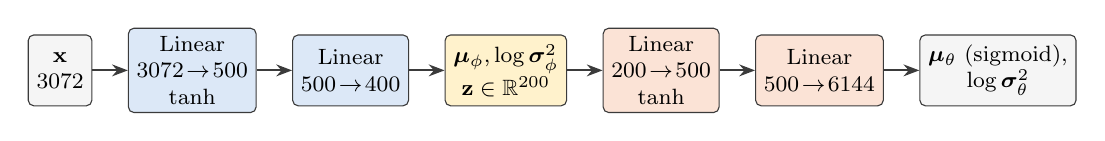
\begin{tikzpicture}[
  box/.style={draw=lineC,rounded corners=2pt,minimum height=0.9cm,align=center,font=\footnotesize,inner sep=3pt},
  ar/.style={-{Stealth[length=2mm]},thick,lineC}]
\node[box,fill=gray!8] (x) {$\x$\\$3072$};
\node[box,fill=encC,right=0.45cm of x] (h1) {Linear\\$3072\!\to\!500$\\$\tanh$};
\node[box,fill=encC,right=0.45cm of h1] (h2) {Linear\\$500\!\to\!400$};
\node[box,fill=latC,right=0.45cm of h2] (z) {$\mub_\phi,\log\sigb^2_\phi$\\$\z\in\mathbb{R}^{200}$};
\node[box,fill=decC,right=0.45cm of z] (d1) {Linear\\$200\!\to\!500$\\$\tanh$};
\node[box,fill=decC,right=0.45cm of d1] (d2) {Linear\\$500\!\to\!6144$};
\node[box,fill=gray!8,right=0.45cm of d2] (out) {$\mub_\theta$ (sigmoid),\\$\log\sigb^2_\theta$};
\foreach \a/\b in {x/h1,h1/h2,h2/z,z/d1,d1/d2,d2/out} \draw[ar] (\a) -- (\b);
\end{tikzpicture}
\caption{VAE-MLP: one $\tanh$ hidden layer of 500 units on each side, as in \citet{kingma2014vae}.}
\label{fig:arch-mlp}
\end{figure}

The image is flattened into a vector of $D=3072$ values, so the network has no notion of spatial neighbourhood.
Following the paper's Gaussian MLP (Appendix~C.2):
\begin{align}
  \text{encoder:}\quad & \mathbf{h} = \tanh(\mathbf{W}_1\x + \mathbf{b}_1),\qquad
                         [\mub_\phi,\log\sigb^2_\phi] = \mathbf{W}_2\mathbf{h} + \mathbf{b}_2,\\
  \text{decoder:}\quad & \mathbf{h}' = \tanh(\mathbf{W}_3\z + \mathbf{b}_3),\qquad
                         [\mathbf{m},\mathbf{r}] = \mathbf{W}_4\mathbf{h}'+\mathbf{b}_4,\qquad
                         \mub_\theta = 2\,\mathrm{sigmoid}(\mathbf{m})-1.
\end{align}
The sigmoid constrains the decoder means, as in the paper; the factor $2(\cdot)-1$ maps it to our $[-1,1]$ pixel
range. The decoder log-variance $\mathbf{r}$ is used through the soft lower bound described in
\cref{sec:arch-conv}. All parameters are initialised from $\N(0,0.01^2)$.

\begin{table}[H]
\centering\small
\caption{VAE-MLP layers. Total: \textbf{4,915,544} parameters.}
\label{tab:arch-mlp}
\begin{tabular}{@{}llrr@{}}
\toprule
Part & Layer & Output & Parameters\\
\midrule
Encoder & Flatten & $3072$ & 0\\
        & Linear $3072\to500$, $\tanh$ & $500$ & 1,536,500\\
        & Linear $500\to2\times200$ ($\mub_\phi$, $\log\sigb_\phi^2$) & $2\times200$ & 200,400\\
\midrule
Decoder & Linear $200\to500$, $\tanh$ & $500$ & 100,500\\
        & Linear $500\to2\times3072$ ($\mub_\theta$, $\log\sigb_\theta^2$) & $2\times3\times32\times32$ & 3,078,144\\
\bottomrule
\end{tabular}
\end{table}

\subsection{Model B --- VAE-Conv: the same method with a convolutional network}
\label{sec:arch-conv}

\begin{figure}[H]
\centering
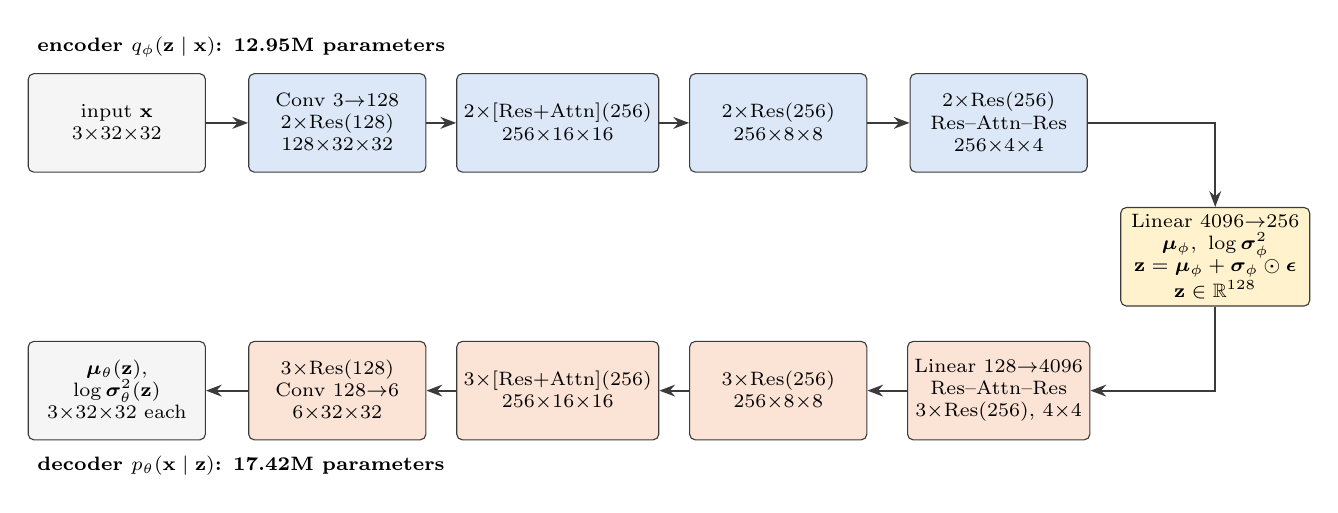
\begin{tikzpicture}[
  stage/.style={draw=lineC,rounded corners=2pt,align=center,font=\scriptsize,inner sep=2.5pt,minimum width=2.25cm,minimum height=1.25cm},
  ar/.style={-{Stealth[length=2mm]},thick,lineC}]
% encoder (top row, left to right)
\node[stage,fill=gray!8] (in) at (0,0) {input $\x$\\$3{\times}32{\times}32$};
\node[stage,fill=encC] (e0) at (2.8,0) {Conv $3{\to}128$\\2$\times$Res(128)\\$128{\times}32{\times}32$};
\node[stage,fill=encC] (e1) at (5.6,0) {2$\times$[Res+Attn](256)\\$256{\times}16{\times}16$};
\node[stage,fill=encC] (e2) at (8.4,0) {2$\times$Res(256)\\$256{\times}8{\times}8$};
\node[stage,fill=encC] (e3) at (11.2,0) {2$\times$Res(256)\\Res--Attn--Res\\$256{\times}4{\times}4$};
% latent
\node[stage,fill=latC,minimum width=2.4cm] (z) at (13.95,-1.7)
  {Linear $4096{\to}256$\\$\mub_\phi,\ \log\sigb^2_\phi$\\$\z=\mub_\phi+\sigb_\phi\odot\eps$\\$\z\in\mathbb{R}^{128}$};
% decoder (bottom row, right to left)
\node[stage,fill=decC] (d3) at (11.2,-3.4) {Linear $128{\to}4096$\\Res--Attn--Res\\3$\times$Res(256), $4{\times}4$};
\node[stage,fill=decC] (d2) at (8.4,-3.4) {3$\times$Res(256)\\$256{\times}8{\times}8$};
\node[stage,fill=decC] (d1) at (5.6,-3.4) {3$\times$[Res+Attn](256)\\$256{\times}16{\times}16$};
\node[stage,fill=decC] (d0) at (2.8,-3.4) {3$\times$Res(128)\\Conv $128{\to}6$\\$6{\times}32{\times}32$};
\node[stage,fill=gray!8] (out) at (0,-3.4) {$\mub_\theta(\z)$,\\$\log\sigb^2_\theta(\z)$\\$3{\times}32{\times}32$ each};
\foreach \a/\b in {in/e0,d3/d2,d2/d1,d1/d0,d0/out} \draw[ar] (\a) -- (\b);
\draw[ar] (e0) -- (e1);
\draw[ar] (e1) -- (e2);
\draw[ar] (e2) -- (e3);
\draw[ar] (e3.east) -| (z.north);
\draw[ar] (z.south) |- (d3.east);
\node[font=\scriptsize\bfseries,anchor=south west] at ($(in.north west)+(0,0.08)$) {encoder $q_\phi(\z\mid\x)$: 12.95M parameters};
\node[font=\scriptsize\bfseries,anchor=north west] at ($(out.south west)+(0,-0.08)$) {decoder $p_\theta(\x\mid\z)$: 17.42M parameters};
\end{tikzpicture}
\caption{VAE-Conv. The encoder (top) mirrors the U-Net's downsampling path and the decoder (bottom) its upsampling
path, using the same blocks and widths but \emph{without skip connections}: all information must pass through the
128-d latent $\z$ (right).}
\label{fig:arch-conv}
\end{figure}

A one-layer MLP has $4.9$M parameters and no spatial inductive bias. Compared with a $35.7$M-parameter U-Net, it
would turn the comparison into ``MLP vs.\ U-Net''. VAE-Conv therefore keeps the VAE \emph{method} of
\cref{sec:bg-vae} exactly and replaces only the \emph{network}, with an encoder and decoder built from the blocks
of \cref{sec:blocks} at the U-Net's widths (base width $128$, channel multipliers $(1,2,2,2)$, two residual blocks
per level, attention at $16\times16$).

\paragraph{Encoder, step by step.}
\begin{enumerate}
  \item A $3\times3$ convolution lifts the image to $128$ channels.
  \item Four resolution levels ($32\to16\to8\to4$) apply two residual blocks each; the $16\times16$ level adds
        self-attention after each block.
  \item Stride-2 convolutions downsample between levels.
  \item A bottleneck (residual block, attention, residual block) operates at $4\times4$.
  \item GroupNorm and SiLU are applied, and the result is flattened to $256\cdot4\cdot4=4096$ values.
  \item A linear layer outputs $\mub_\phi(\x)$ and $\log\sigb^2_\phi(\x)$ ($2\times128$ values). The latent is
        sampled with the reparameterisation trick.
\end{enumerate}

\paragraph{Decoder, step by step.}
\begin{enumerate}
  \item A linear layer maps $\z\in\mathbb{R}^{128}$ to a $256\times4\times4$ tensor.
  \item The same bottleneck is applied.
  \item Four levels with \emph{three} residual blocks each (mirroring the U-Net's upsampling path) upsample back to
        $32\times32$.
  \item GroupNorm, SiLU and a $3\times3$ convolution produce $6$ channels: the per-pixel mean $\mub_\theta(\z)$
        and raw log-variance $\mathbf{r}(\z)$ of the Gaussian decoder.
\end{enumerate}

\paragraph{Decoder variance.} With dequantised data, a log-variance far below the variance of the dequantisation
noise brings no real gain in likelihood and is numerically unstable. We therefore use a soft lower bound,
\begin{equation}
  \log\sigb^2_\theta(\z) = \ell_{\min} + \operatorname{softplus}\big(\mathbf{r}(\z)-\ell_{\min}\big),
  \qquad \ell_{\min}=-12,
\end{equation}
which lies at the level of the dequantisation noise. The same bound is used in VAE-MLP.

\begin{table}[t]
\centering\small
\caption{VAE-Conv layers (output shapes are channels $\times$ height $\times$ width). Encoder 12,950,400 +
decoder 17,421,190 = \textbf{30,371,590} parameters.}
\label{tab:arch-conv}
\begin{tabular}{@{}llrr@{}}
\toprule
Part & Stage & Output & Parameters\\
\midrule
\multirow{8}{*}{Encoder}
 & Conv $3\times3$, $3\to128$ & $128\times32\times32$ & 3,584\\
 & Level 0: 2$\times$Res(128) + downsample & $128\times16\times16$ & 738,944\\
 & Level 1: 2$\times$[Res + Attn](256) + downsample & $256\times8\times8$ & 3,217,664\\
 & Level 2: 2$\times$Res(256) + downsample & $256\times4\times4$ & 2,952,448\\
 & Level 3: 2$\times$Res(256) & $256\times4\times4$ & 2,362,368\\
 & Bottleneck: Res -- Attn -- Res & $256\times4\times4$ & 2,626,048\\
 & GN, SiLU, flatten & $4096$ & 512\\
 & Linear $4096\to2\times128$ ($\mub_\phi$, $\log\sigb^2_\phi$) & $2\times128$ & 1,048,832\\
\midrule
\multirow{7}{*}{Decoder}
 & Linear $128\to4096$, reshape & $256\times4\times4$ & 528,384\\
 & Bottleneck: Res -- Attn -- Res & $256\times4\times4$ & 2,626,048\\
 & Level 3: 3$\times$Res(256) + upsample & $256\times8\times8$ & 4,133,632\\
 & Level 2: 3$\times$Res(256) + upsample & $256\times16\times16$ & 4,133,632\\
 & Level 1: 3$\times$[Res + Attn](256) + upsample & $256\times32\times32$ & 4,924,672\\
 & Level 0: 3$\times$Res(128) & $128\times32\times32$ & 1,067,648\\
 & GN, SiLU, Conv $3\times3$, $128\to6$ ($\mub_\theta$, $\mathbf{r}$) & $6\times32\times32$ & 7,174\\
\bottomrule
\end{tabular}
\end{table}

\subsection{Model C --- DDPM: the noise-prediction U-Net of Ho et al.}
\label{sec:arch-unet}

\begin{figure}[H]
\centering
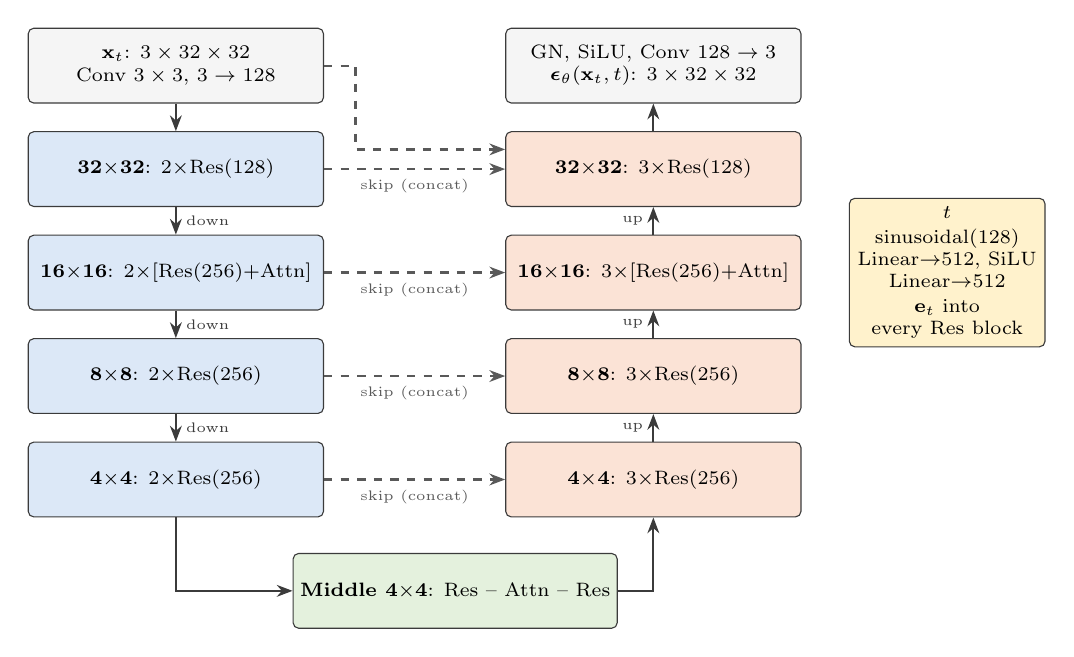
\begin{tikzpicture}[
  stage/.style={draw=lineC,rounded corners=2pt,align=center,font=\scriptsize,inner sep=2.5pt,minimum width=3.75cm,minimum height=0.95cm},
  ar/.style={-{Stealth[length=2mm]},thick,lineC},
  skip/.style={-{Stealth[length=2mm]},thick,dashed,gray!70!black}]
\node[stage,fill=gray!8] (in) {$\x_t$: $3\times32\times32$\\Conv $3\times3$, $3\to128$};
\node[stage,fill=encC,below=0.35cm of in] (d0) {\textbf{32$\times$32}: 2$\times$Res(128)};
\node[stage,fill=encC,below=0.35cm of d0] (d1) {\textbf{16$\times$16}: 2$\times$[Res(256)+Attn]};
\node[stage,fill=encC,below=0.35cm of d1] (d2) {\textbf{8$\times$8}: 2$\times$Res(256)};
\node[stage,fill=encC,below=0.35cm of d2] (d3) {\textbf{4$\times$4}: 2$\times$Res(256)};
\node[stage,fill=midC,below right=0.45cm and -0.4cm of d3,minimum width=3.9cm] (mid) {\textbf{Middle 4$\times$4}: Res -- Attn -- Res};
\node[stage,fill=decC,right=2.3cm of d3] (u3) {\textbf{4$\times$4}: 3$\times$Res(256)};
\node[stage,fill=decC,above=0.35cm of u3] (u2) {\textbf{8$\times$8}: 3$\times$Res(256)};
\node[stage,fill=decC,above=0.35cm of u2] (u1) {\textbf{16$\times$16}: 3$\times$[Res(256)+Attn]};
\node[stage,fill=decC,above=0.35cm of u1] (u0) {\textbf{32$\times$32}: 3$\times$Res(128)};
\node[stage,fill=gray!8,above=0.35cm of u0] (out) {GN, SiLU, Conv $128\to3$\\$\eps_\theta(\x_t,t)$: $3\times32\times32$};
\draw[ar] (in) -- (d0);
\draw[ar] (d0) -- node[right,font=\tiny]{down} (d1);
\draw[ar] (d1) -- node[right,font=\tiny]{down} (d2);
\draw[ar] (d2) -- node[right,font=\tiny]{down} (d3);
\draw[ar] (d3.south) |- (mid.west);
\draw[ar] (mid.east) -| (u3.south);
\draw[ar] (u3) -- node[left,font=\tiny]{up} (u2);
\draw[ar] (u2) -- node[left,font=\tiny]{up} (u1);
\draw[ar] (u1) -- node[left,font=\tiny]{up} (u0);
\draw[ar] (u0) -- (out);
\foreach \a/\b in {d0/u0,d1/u1,d2/u2,d3/u3} \draw[skip] (\a.east) -- node[below,font=\tiny]{skip (concat)} (\b.west);
\draw[skip] (in.east) -- ++(0.4,0) |- ($(u0.west)+(0,0.25)$);
\node[draw=lineC,fill=latC,rounded corners=2pt,font=\scriptsize,align=center,right=0.6cm of u1,inner sep=3pt] (t)
  {$t$\\[1pt]sinusoidal(128)\\Linear$\to$512, SiLU\\Linear$\to$512\\[1pt]$\mathbf{e}_t$ into\\every Res block};
\end{tikzpicture}
\caption{The DDPM U-Net~\citep{ronneberger2015unet,salimans2017pixelcnnpp}. The left path stores 12 activations
(the input convolution, every residual block and every downsampling). The right path concatenates one of them
before each of its residual blocks (dashed arrows; one is drawn per level). The timestep embedding
$\mathbf{e}_t$ conditions every residual block. Total: 35,746,307 parameters.}
\label{fig:arch-unet}
\end{figure}

The DDPM network $\eps_\theta(\x_t,t)$ maps a noisy image and its timestep to a prediction of the added noise, so
input and output have the same shape. We reproduce the CIFAR-10 configuration of \citet{ho2020ddpm}
(Appendix~B): a PixelCNN++-style U-Net on a Wide-ResNet backbone with GroupNorm, four resolutions, two residual
blocks per level on the way down, self-attention at $16\times16$, dropout $0.1$, and the sinusoidal timestep
embedding added to every residual block.

\paragraph{How the U-Net processes an input, step by step.}
\begin{enumerate}
  \item \textbf{Time conditioning.} $t$ is embedded into $\mathbf{e}_t\in\mathbb{R}^{512}$, which every residual
        block adds after its first convolution (\cref{eq:res1}). One set of weights can therefore denoise at all
        $1000$ noise levels.
  \item \textbf{Contracting path.} A $3\times3$ convolution lifts $\x_t$ to $128$ channels. Four levels
        ($32,16,8,4$) each apply two residual blocks, with attention at $16\times16$, followed by stride-2
        downsampling. Every intermediate activation is stored for later.
  \item \textbf{Middle.} A residual block, global self-attention and another residual block at $4\times4$ give
        every position a view of the whole image.
  \item \textbf{Expanding path.} At each level, three residual blocks each take the current features
        \emph{concatenated} with one stored activation of the same resolution. This is why their input widths
        (e.g.\ $512=256+256$ or $384=256+128$) exceed their outputs. Nearest-neighbour upsampling with a
        convolution doubles the resolution between levels.
  \item \textbf{Output.} GroupNorm, SiLU and a zero-initialised $3\times3$ convolution produce
        $\eps_\theta(\x_t,t)$.
\end{enumerate}
The skip connections are the key structural difference from VAE-Conv. They let fine detail bypass the bottleneck,
which is appropriate here because the DDPM never needs to compress: its ``latent'' $\x_t$ is as large as the image.

\begin{table}[t]
\centering\small
\caption{DDPM U-Net (CIFAR-10 configuration). Residual blocks on the expanding path receive concatenated skip
features, so their input width is shown as $C_\text{in}\!\to\!C_\text{out}$. Total: \textbf{35,746,307}
parameters (paper: 35.7M).}
\label{tab:arch-unet}
\begin{tabular}{@{}llrr@{}}
\toprule
Path & Stage & Output & Parameters\\
\midrule
 & Timestep MLP: sinusoidal(128) $\to$ 512 $\to$ 512 & $512$ & 328,704\\
 & Conv $3\times3$, $3\to128$ & $128\times32\times32$ & 3,584\\
\midrule
\multirow{4}{*}{Down}
 & 32$\times$32: 2$\times$Res $128\to128$ + downsample & $128\times16\times16$ & 870,272\\
 & 16$\times$16: 2$\times$[Res + Attn], $128\to256$ + downsample & $256\times8\times8$ & 3,480,320\\
 & 8$\times$8: 2$\times$Res $256\to256$ + downsample & $256\times4\times4$ & 3,215,104\\
 & 4$\times$4: 2$\times$Res $256\to256$ & $256\times4\times4$ & 2,625,024\\
\midrule
Middle & Res -- Attn -- Res (256) & $256\times4\times4$ & 2,888,704\\
\midrule
\multirow{4}{*}{Up}
 & 4$\times$4: 3$\times$Res $512\to256$ + upsample & $256\times8\times8$ & 6,692,608\\
 & 8$\times$8: 3$\times$Res $512\to256$ + upsample & $256\times16\times16$ & 6,692,608\\
 & 16$\times$16: 3$\times$[Res + Attn] ($512,512,384\to256$) + upsample & $256\times32\times32$ & 7,155,712\\
 & 32$\times$32: 3$\times$Res ($384,256,256\to128$) & $128\times32\times32$ & 1,789,952\\
\midrule
 & GN, SiLU, Conv $3\times3$, $128\to3$ & $3\times32\times32$ & 3,715\\
\bottomrule
\end{tabular}
\end{table}

\subsection{The three architectures side by side}
\label{sec:arch-compare}

\begin{table}[H]
\centering\small
\caption{Structural comparison of the three models.}
\label{tab:arch-compare}
\begin{tabularx}{\textwidth}{@{}l>{\raggedright\arraybackslash}X>{\raggedright\arraybackslash}X>{\raggedright\arraybackslash}X@{}}
\toprule
 & \textbf{VAE-MLP} & \textbf{VAE-Conv} & \textbf{DDPM}\\
\midrule
Network & 2 hidden layers (1 per side), $\tanh$ & 24 residual + 7 attention blocks, GN + SiLU & U-Net: 22 residual + 6 attention blocks\\
Parameters & 4.9M & 30.4M & 35.7M\\
Spatial inductive bias & none (flattened pixels) & convolutions + attention & convolutions + attention\\
Encoder & learned, amortised & learned, amortised & fixed (Gaussian noising), no parameters\\
Latent & $\z\in\mathbb{R}^{200}$ (compressed $15\times$) & $\z\in\mathbb{R}^{128}$ (compressed $24\times$) & $\x_1,\dots,\x_{1000}$, each $\in\mathbb{R}^{3072}$\\
Skip connections & no & no (bottleneck) & yes (12 U-Net skips)\\
Conditioning & none & none & timestep $t$ in every block\\
Network evaluations per sample & 1 & 1 & 1000 (10--250 with DDIM)\\
Training objective & ELBO, $\beta=1$ & ELBO, $\beta=1$ & $L_\text{simple}$ (reweighted ELBO)\\
\bottomrule
\end{tabularx}
\end{table}

VAE-MLP and VAE-Conv share every component of the method and differ \emph{only} in the network, so comparing them
isolates the effect of architecture. VAE-Conv and the DDPM share building blocks, widths and training settings and
differ in the \emph{generative approach}, so comparing them isolates the effect of VAE versus diffusion.

\section{Training Procedure}
\label{sec:training}

\subsection{Algorithms}
\Cref{alg:vae-train,alg:ddpm-train,alg:ddpm-sample,alg:ddim} summarise how each model is trained and sampled.
All three models use the same training loop (\texttt{src/genmodels/trainer.py}), with bf16 mixed precision,
gradient clipping, an exponential moving average (EMA) of the weights, and checkpoints that can be resumed exactly.

\begin{algorithm}[H]
\caption{VAE training (one step, both VAE variants)}
\label{alg:vae-train}
\begin{algorithmic}[1]
\State Sample a minibatch of pixel values $\{k^{(b)}\}_{b=1}^{B}$
\State Dequantise: $\x^{(b)} \gets (k^{(b)}+\mathbf{u})/128-1$, $\;\mathbf{u}\sim\mathcal{U}[0,1)^{D}$
\State Encode: $\mub_\phi,\log\sigb^2_\phi \gets \mathrm{Enc}_\phi(\x^{(b)})$
\State Reparameterise: $\z \gets \mub_\phi + \sigb_\phi\odot\eps$, $\;\eps\sim\N(\mathbf{0},\I)$
\State Decode: $\mub_\theta,\log\sigb^2_\theta \gets \mathrm{Dec}_\theta(\z)$
\State $\mathcal{B}^{(b)} \gets$ reconstruction term \eqref{eq:vae-recon} $+$ KL term \eqref{eq:vae-kl} \Comment{both summed over all dimensions}
\State Gradient step on $\frac{1}{BD}\sum_b \mathcal{B}^{(b)}$; update the EMA weights
\end{algorithmic}
\end{algorithm}

\begin{algorithm}[H]
\caption{DDPM training with $L_\text{simple}$~\citep{ho2020ddpm}}
\label{alg:ddpm-train}
\begin{algorithmic}[1]
\State Sample a minibatch $\x_0$ (scaled to $[-1,1]$, random horizontal flips)
\State $t\sim\mathcal{U}\{1,\dots,T\}$, $\;\eps\sim\N(\mathbf{0},\I)$ \Comment{independently for each image}
\State $\x_t \gets \sqrt{\abar_t}\,\x_0 + \sqrt{1-\abar_t}\,\eps$ \Comment{\cref{eq:q-marginal}: one shot, no chain}
\State Gradient step on $\big\|\eps-\eps_\theta(\x_t,t)\big\|^2$; update the EMA weights
\end{algorithmic}
\end{algorithm}

\begin{algorithm}[H]
\caption{DDPM ancestral sampling (paper's sampler, $T=1000$ network evaluations)}
\label{alg:ddpm-sample}
\begin{algorithmic}[1]
\State $\x_T\sim\N(\mathbf{0},\I)$
\For{$t=T,\dots,1$}
  \State $\hat\x_0 \gets \operatorname{clip}_{[-1,1]}\!\big((\x_t-\sqrt{1-\abar_t}\,\eps_\theta(\x_t,t))/\sqrt{\abar_t}\big)$
  \State $\x_{t-1} \gets \mutil_t(\x_t,\hat\x_0) + \sigma_t\,\mathbf{z}$, $\;\mathbf{z}\sim\N(\mathbf{0},\I)$ if $t>1$, else $\mathbf{z}=\mathbf{0}$ \Comment{\cref{eq:posterior}}
\EndFor
\State \Return $\x_0$
\end{algorithmic}
\end{algorithm}

\begin{algorithm}[H]
\caption{DDIM sampling~\citep{song2021ddim} ($\eta=0$, $S$ steps, same trained network)}
\label{alg:ddim}
\begin{algorithmic}[1]
\State $\tau \gets (0, c, 2c, \dots)$ with $c=T/S$; $\;\x\sim\N(\mathbf{0},\I)$
\For{$i=S,\dots,1$}
  \State $\hat\eps \gets \eps_\theta(\x,\tau_i)$, $\;\hat\x_0\gets\operatorname{clip}\big((\x-\sqrt{1-\abar_{\tau_i}}\hat\eps)/\sqrt{\abar_{\tau_i}}\big)$
  \State $\hat\eps \gets (\x-\sqrt{\abar_{\tau_i}}\,\hat\x_0)/\sqrt{1-\abar_{\tau_i}}$ \Comment{keep $\hat\eps$ consistent with the clipped $\hat\x_0$}
  \State $\x \gets \sqrt{\abar_{\tau_{i-1}}}\,\hat\x_0 + \sqrt{1-\abar_{\tau_{i-1}}}\,\hat\eps$ \Comment{\cref{eq:ddim}; $\abar_{\tau_0}\!:=\!1$}
\EndFor
\State \Return $\x$
\end{algorithmic}
\end{algorithm}

\subsection{Hyper-parameters and compute}

\begin{table}[H]
\centering\small
\caption{Training configuration (\texttt{configs/*.yaml}). The DDPM settings are those of \citet{ho2020ddpm}
except the number of steps. VAE-Conv uses the DDPM's optimisation settings, for fairness. VAE-MLP uses the
settings of \citet{kingma2014vae}.}
\label{tab:hparams}
\footnotesize
\begin{tabular}{@{}lccc@{}}
\toprule
 & \textbf{VAE-MLP} & \textbf{VAE-Conv} & \textbf{DDPM}\\
\midrule
Optimiser & Adagrad, lr $0.02$ & Adam, lr $2\!\times\!10^{-4}$ & Adam, lr $2\!\times\!10^{-4}$\\
Warm-up / gradient clipping & -- / -- & 5k steps / 1.0 & 5k steps / 1.0\\
Batch size & 100 & 128 & 128\\
Training steps (epochs) & 500k (1000) & 60k (154) & 150k (384); paper: 800k\\
Regularisation & weight decay from $p(\theta)=\N(\mathbf{0},\I)$ & -- & dropout 0.1\\
Augmentation & none & horizontal flips & horizontal flips\\
EMA decay & 0.9999 & 0.9999 & 0.9999\\
Initialisation & $\N(0,0.01^2)$ & Xavier (fan-avg) & Xavier (fan-avg)\\
Precision & fp32 & bf16 autocast & bf16 autocast\\
Training time (A100-80GB) & 0.44\,h & 1.32\,h & 3.94\,h\\
\bottomrule
\end{tabular}
\end{table}

All models were trained on a single NVIDIA A100-SXM4-80GB (Google Colab). The total training compute was
$5.72$ GPU-hours, including a $0.02$-hour CIFAR-10 classifier used as an evaluation instrument.

The DDPM is the only model whose training length deviates from its paper: $150$k instead of $800$k steps, which
the compute budget required. For reference, \citet{ho2020ddpm} trained for 10.6 hours on a TPU v3-8, roughly
comparable to 8 V100 GPUs. \Cref{sec:limitations} discusses the effect on the results.

\section{Evaluation Protocol}
\label{sec:eval}

Every model is evaluated by the same script (\texttt{scripts/evaluate.py}) on the same GPU.
\begin{itemize}
  \item Each sample set has $N=10{,}000$ images.
  \item The reference set is the $50{,}000$ CIFAR-10 training images.
  \item FID, IS, KID and precision/recall all use the same Inception-v3 features: the TF-compatible network of
        \texttt{torch-fidelity}~\citep{obukhov2020torchfidelity}.
\end{itemize}

\subsection{Metrics}
Let $\{\mathbf{f}_i\}$ denote 2048-d Inception pool features of real ($r$) or generated ($g$) images.
\begin{itemize}
  \item \textbf{Fréchet Inception Distance}~\citep{heusel2017fid}: the distance between Gaussians fitted to the
        two feature sets. It measures quality and diversity together.
  \begin{equation}
    \mathrm{FID} = \|\mathbf{m}_r-\mathbf{m}_g\|_2^2 + \Tr\!\Big(\bm{\Sigma}_r+\bm{\Sigma}_g-2\big(\bm{\Sigma}_r\bm{\Sigma}_g\big)^{1/2}\Big).
  \end{equation}
  \item \textbf{Inception Score}~\citep{salimans2016improved}: high when each image is classified confidently and
        the classes are varied. It never compares against real CIFAR-10 images. 10 splits:
  \begin{equation}
    \mathrm{IS} = \exp\Big(\E_{\x}\,\KL{p(y\mid\x)}{p(y)}\Big).
  \end{equation}
  \item \textbf{Kernel Inception Distance}~\citep{binkowski2018kid}: an unbiased estimate of the squared MMD with
        kernel $k(\mathbf{a},\mathbf{b})=(\mathbf{a}^\top\mathbf{b}/2048+1)^3$, averaged over 100 subsets of 1000.
        Unlike FID, it is unbiased at our sample size.
  \item \textbf{Precision and recall}~\citep{kynkaanniemi2019pr}: each real feature is assigned a radius equal to
        the distance to its $k$-th nearest real neighbour ($k=3$), and likewise for generated features.
  \begin{equation}
    \mathrm{precision} = \frac{1}{N_g}\sum_{j}\mathbb{1}\big[\mathbf{f}^g_j \in \textstyle\bigcup_i B(\mathbf{f}^r_i, r_i)\big],\qquad
    \mathrm{recall} = \frac{1}{N_r}\sum_{i}\mathbb{1}\big[\mathbf{f}^r_i \in \textstyle\bigcup_j B(\mathbf{f}^g_j, r_j)\big].
  \end{equation}
        Precision measures \emph{realism}: generated images lie on the real data manifold. Recall measures
        \emph{diversity}: generated images cover the real data. FID mixes the two.
  \item \textbf{Likelihood}: the test-set negative ELBO in bits/dim, using \cref{eq:bpd} for the VAEs and the full
        bound of \cref{eq:vlb} for the DDPM. Both are upper bounds on the negative log-likelihood of the discrete
        data, so they are directly comparable.
  \item \textbf{Cost}: network evaluations per image (NFE, hardware-independent), throughput in images/s at batch
        256, and single-image latency, all in bf16 on the A100.
  \item \textbf{Thematic consistency}: a ResNet-18 trained from scratch on CIFAR-10 ($93.6\%$ test accuracy)
        labels every generated image. We report its mean confidence, the share of confident predictions
        ($>0.9$), and the normalised entropy of the predicted-class histogram ($1$ = all classes equally frequent).
  \item \textbf{Memorisation}: for every sample, the Inception-feature distance to its nearest training image,
        relative to the same distance for unseen real test images.
\end{itemize}

\subsection{Protocol and fairness}
\begin{itemize}
  \item \textbf{Validated metrics.} On real data, our pipeline gives $\mathrm{FID}(\text{test}_{10\text{k}},
        \text{train}_{50\text{k}})=3.15$ and $\mathrm{IS}(\text{test})=10.97$, matching published reference
        values. This was checked before any model was evaluated.
  \item \textbf{Real-data reference row.} Every metric is also reported for real test images, so the ceiling is
        visible.
  \item \textbf{Fixed checkpoints, no cherry-picking.} The final EMA checkpoint of each run was chosen before
        evaluation, and all sample grids are uncurated.
  \item \textbf{Evaluation noise.} Headline settings are evaluated on three independent sample sets and reported
        as mean $\pm$ standard deviation.
  \item \textbf{Same conditions.} All models use identical data, preprocessing, GPU and software.
\end{itemize}

\section{Quantitative Results}
\label{sec:results}

\subsection{Main comparison}

\begin{table}[H]
\centering\footnotesize
\setlength{\tabcolsep}{3.5pt}
\caption{Main results ($N=10{,}000$ samples against the CIFAR-10 training set). $\pm$: standard deviation over three
independent sample sets (evaluation noise). NFE: network evaluations per image. Bits/dim: test-set bound; it is a
property of the model, so both DDPM rows share it.}
\label{tab:main}
\resizebox{\textwidth}{!}{%
\begin{tabular}{@{}lccccccrr@{}}
\toprule
Model & FID$\downarrow$ & IS$\uparrow$ & KID$\times10^3\!\downarrow$ & Prec.$\uparrow$ & Rec.$\uparrow$ & Bits/dim$\downarrow$ & NFE & Img/s$\uparrow$\\
\midrule
\textit{Real test images} & \textit{3.15} & \textit{10.97} & \textit{$-$0.01} & \textit{0.681} & \textit{0.693} & -- & -- & --\\
VAE-MLP & 135.97\,$\pm$\,0.52 & 3.11\,$\pm$\,0.02 & 127.57\,$\pm$\,0.62 & 0.323\,$\pm$\,0.006 & 0.003\,$\pm$\,0.001 & 6.313 & 1 & 350{,}102\\
VAE-Conv & 121.85\,$\pm$\,0.30 & 3.88\,$\pm$\,0.05 & 151.18\,$\pm$\,0.45 & 0.404\,$\pm$\,0.010 & 0.073\,$\pm$\,0.020 & 5.826 & 1 & 7{,}017\\
\textbf{DDPM}, 1000 steps & \textbf{6.58} & \textbf{8.59} & \textbf{1.54} & \textbf{0.694} & 0.583 & \textbf{3.794} & 1000 & 4.2\\
DDPM, DDIM 100 steps & 9.66\,$\pm$\,0.06 & 8.31\,$\pm$\,0.10 & 6.35\,$\pm$\,0.14 & 0.641\,$\pm$\,0.007 & \textbf{0.592}\,$\pm$\,0.008 & 3.794 & 100 & 41.6\\
\bottomrule
\end{tabular}}
\end{table}

\begin{itemize}
  \item \textbf{The DDPM wins every quality metric by a wide margin.} Its FID is $18.5\times$ lower than VAE-Conv's
        and its IS $2.2\times$ higher. Its precision ($0.694$) equals that of real images ($0.681$), and its recall
        is $8\times$ VAE-Conv's.
  \item \textbf{The VAE is about $1{,}700\times$ faster} ($7{,}017$ vs.\ $4.2$ images/s; $14$\,ms vs.\ $21.8$\,s for a
        single image).
  \item \textbf{Between the two VAEs,} the convolutional network is better on FID, IS, precision, recall and
        likelihood, but worse on KID. Both VAEs are far from the data distribution, where the metrics stop ranking
        models consistently, so we conclude only that VAE-Conv is better on most measures.
\end{itemize}

\paragraph{Comparison with the original paper.}
\begin{itemize}
  \item \textbf{Likelihood.} After $150$k of the paper's $800$k steps, our DDPM's test bound is $3.794$\,bits/dim
        with $\sigma_t^2=\beta_t$, or $3.781$ with $\sigma_t^2=\btil_t$. The paper reports $\le3.75$ for
        $L_\text{simple}$ (\citealp{ho2020ddpm}, Table~2). Agreement to within $0.04$\,bits/dim is strong evidence
        that the network, schedule and bound are implemented correctly.
  \item \textbf{FID and IS.} The paper reports $3.17$ and $9.46$ with $50$k samples and its best checkpoint. Our
        $6.58$ and $8.59$ use $10$k samples (which raises FID) and the final checkpoint. Training was also $5.3\times$
        shorter, and FID was still falling at the end of training (\cref{fig:fid-train}).
\end{itemize}

\subsection{Speed--quality trade-off}

\begin{figure}[H]
\centering
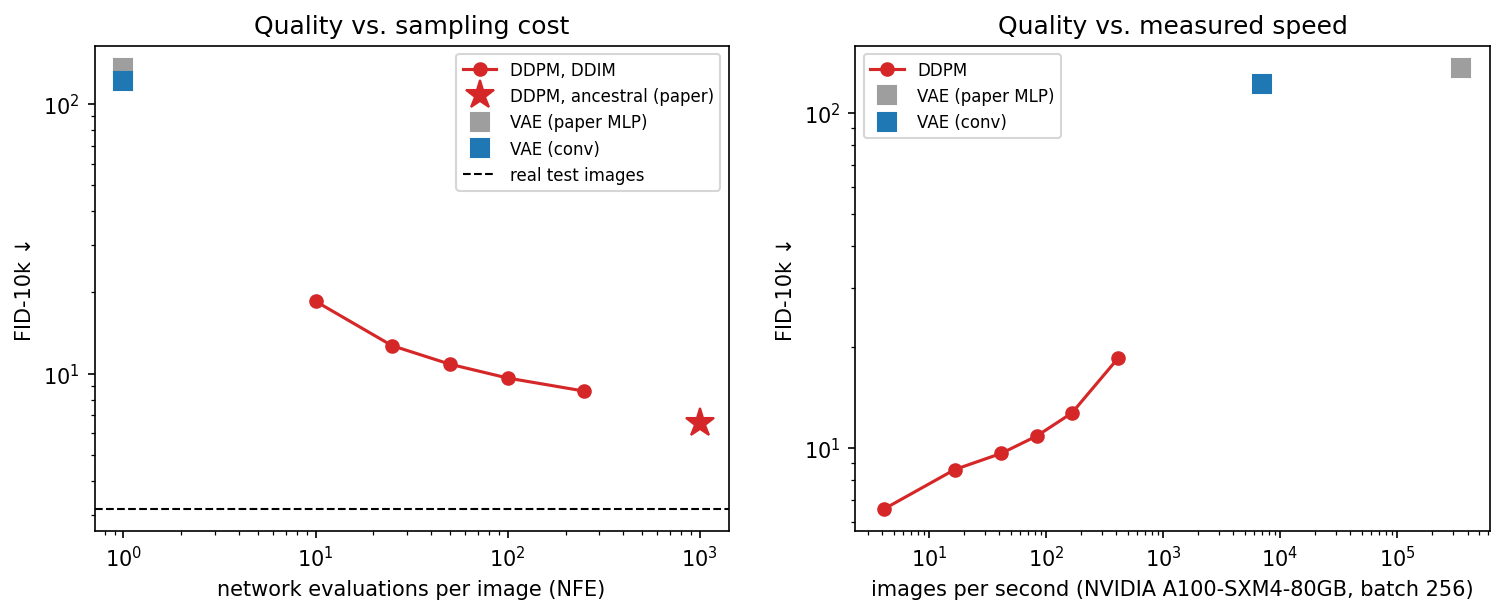
\includegraphics[width=\textwidth]{fig_speed_quality.png}
\caption{Left: FID against the number of network evaluations per image (log--log). Right: FID against measured
throughput. DDIM traces a frontier with the \emph{same} trained DDPM; the VAEs are single points at one
evaluation.}
\label{fig:speed}
\end{figure}

\begin{table}[H]
\centering\small
\caption{DDPM sampling steps (same network; DDIM sets share their starting noise).}
\label{tab:ddim}
\begin{tabular}{@{}lrcccccr@{}}
\toprule
Sampler & NFE & FID$\downarrow$ & IS$\uparrow$ & Precision & Recall & Img/s & Latency (1 image)\\
\midrule
Ancestral (paper) & 1000 & \textbf{6.58} & \textbf{8.59} & \textbf{0.694} & 0.583 & 4.2 & 21.75\,s\\
DDIM & 250 & 8.61 & 8.36 & 0.643 & \textbf{0.595} & 16.6 & 5.41\,s\\
DDIM & 100 & 9.63 & 8.24 & 0.639 & 0.584 & 41.6 & 2.20\,s\\
DDIM & 50 & 10.84 & 8.11 & 0.632 & 0.572 & 83.3 & 1.12\,s\\
DDIM & 25 & 12.70 & 8.02 & 0.626 & 0.555 & 166.5 & 0.55\,s\\
DDIM & 10 & 18.55 & 7.72 & 0.595 & 0.509 & 415.6 & 0.23\,s\\
\midrule
\textit{VAE-Conv} & \textit{1} & \textit{121.85} & \textit{3.88} & \textit{0.404} & \textit{0.073} & \textit{7{,}017} & \textit{14\,ms}\\
\bottomrule
\end{tabular}
\end{table}

\begin{itemize}
  \item DDIM with 10 steps is $100\times$ faster than the paper's sampler and still $6.6\times$ better in FID than
        VAE-Conv.
  \item DDIM does not reach the ancestral sampler's quality even at 250 steps.
  \item No DDPM setting matches the VAE's speed: at 10 steps it is still $17\times$ slower.
\end{itemize}

\subsection{Quality versus diversity}

\begin{figure}[H]
\centering
\begin{minipage}[c]{0.48\textwidth}
\centering
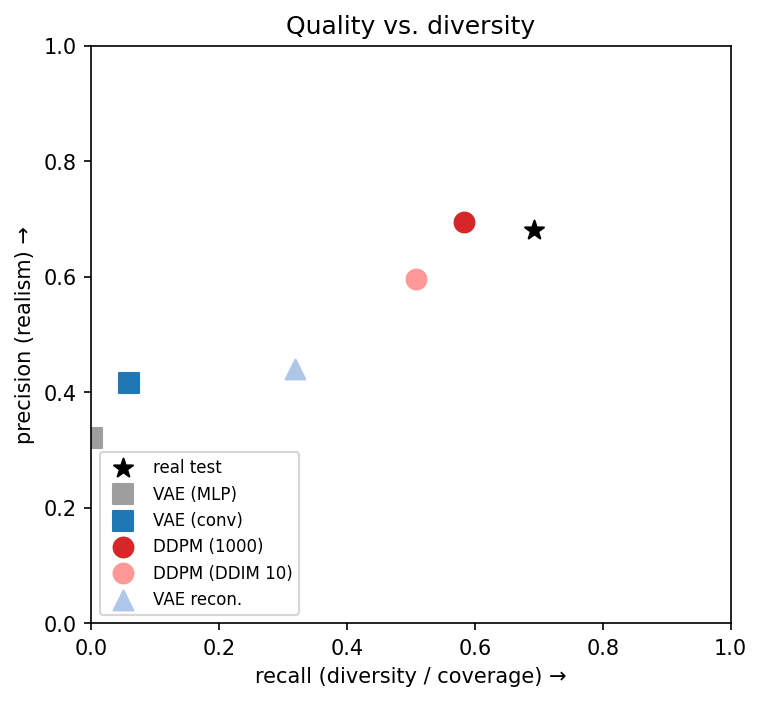
\includegraphics[width=\textwidth]{fig_precision_recall.png}
\end{minipage}\hfill
\begin{minipage}[c]{0.48\textwidth}
\caption{Precision (realism) against recall (diversity), both computed in Inception feature space. Real test
images (star) mark the ceiling. The DDPM sits next to them; both VAEs are in the low-recall corner. VAE-Conv's
reconstructions (triangle) cover far more of the data than its samples do.}
\label{fig:pr}
\end{minipage}
\end{figure}

\begin{figure}[H]
\centering
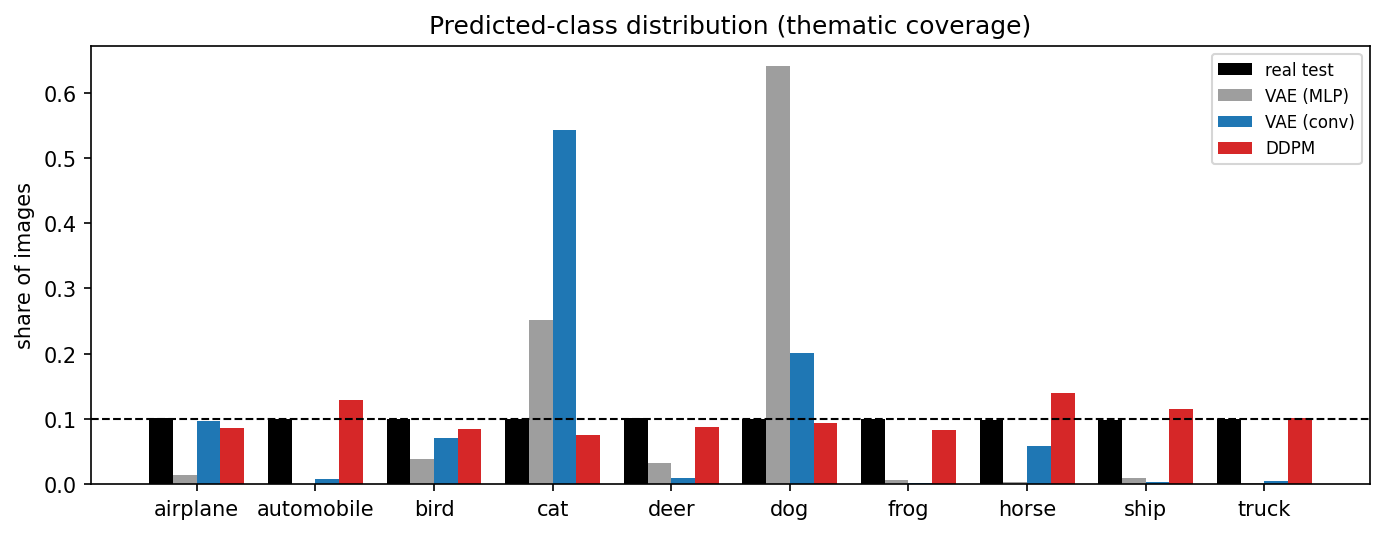
\includegraphics[width=0.92\textwidth]{fig_class_distribution.png}
\caption{Distribution of the classes predicted by the CIFAR-10 classifier for each model's samples. Dashed line:
the uniform share of $0.1$ that real data has.}
\label{fig:classes}
\end{figure}

The DDPM lies next to the real-data point in \cref{fig:pr}, while both VAEs sit in the low-recall corner. The VAEs'
main failure is therefore \emph{coverage}, not only blur. VAE-Conv's \emph{reconstructions} reach a recall of
$0.32$, which points to the cause (\cref{sec:prior-hole}).

\begin{table}[H]
\centering\small
\caption{Thematic consistency, measured by a CIFAR-10 classifier (93.6\% accuracy on real test images).}
\label{tab:thematic}
\begin{tabular}{@{}lcccc@{}}
\toprule
Images & Mean conf.$\uparrow$ & Conf.\ $>0.9\uparrow$ & Class entropy (1 = even) & Rarest class share\\
\midrule
Real test images & 0.875 & 0.742 & 1.000 & 0.098\\
VAE-MLP & 0.756 & 0.298 & 0.455 & 0.000\\
VAE-Conv & 0.692 & 0.164 & 0.601 & 0.003\\
DDPM (1000 steps) & \textbf{0.865} & \textbf{0.719} & \textbf{0.991} & \textbf{0.076}\\
DDPM (DDIM 100) & 0.854 & 0.670 & 0.995 & 0.080\\
\bottomrule
\end{tabular}
\end{table}

\begin{itemize}
  \item \textbf{DDPM samples are almost as recognisable as real photographs} (confidence 0.865 vs.\ 0.875), and all
        ten classes appear in nearly equal shares.
  \item \textbf{The VAEs' class distribution collapses.} The classifier labels $54\%$ of VAE-Conv samples ``cat''
        and $64\%$ of VAE-MLP samples ``dog'', while automobile, frog, ship and truck almost vanish from VAE-Conv's
        samples.
  \item \textbf{This does not mean the VAE ``draws cats''.} Its blurry, brownish samples fall \emph{between}
        classes, and an uncertain classifier assigns them to broad animal classes. Only $16\%$ of VAE-Conv samples
        are classified with confidence above $0.9$, against $72\%$ for the DDPM.
\end{itemize}

\subsection{Training dynamics and the VAE's prior hole}
\label{sec:prior-hole}

\begin{figure}[H]
\centering
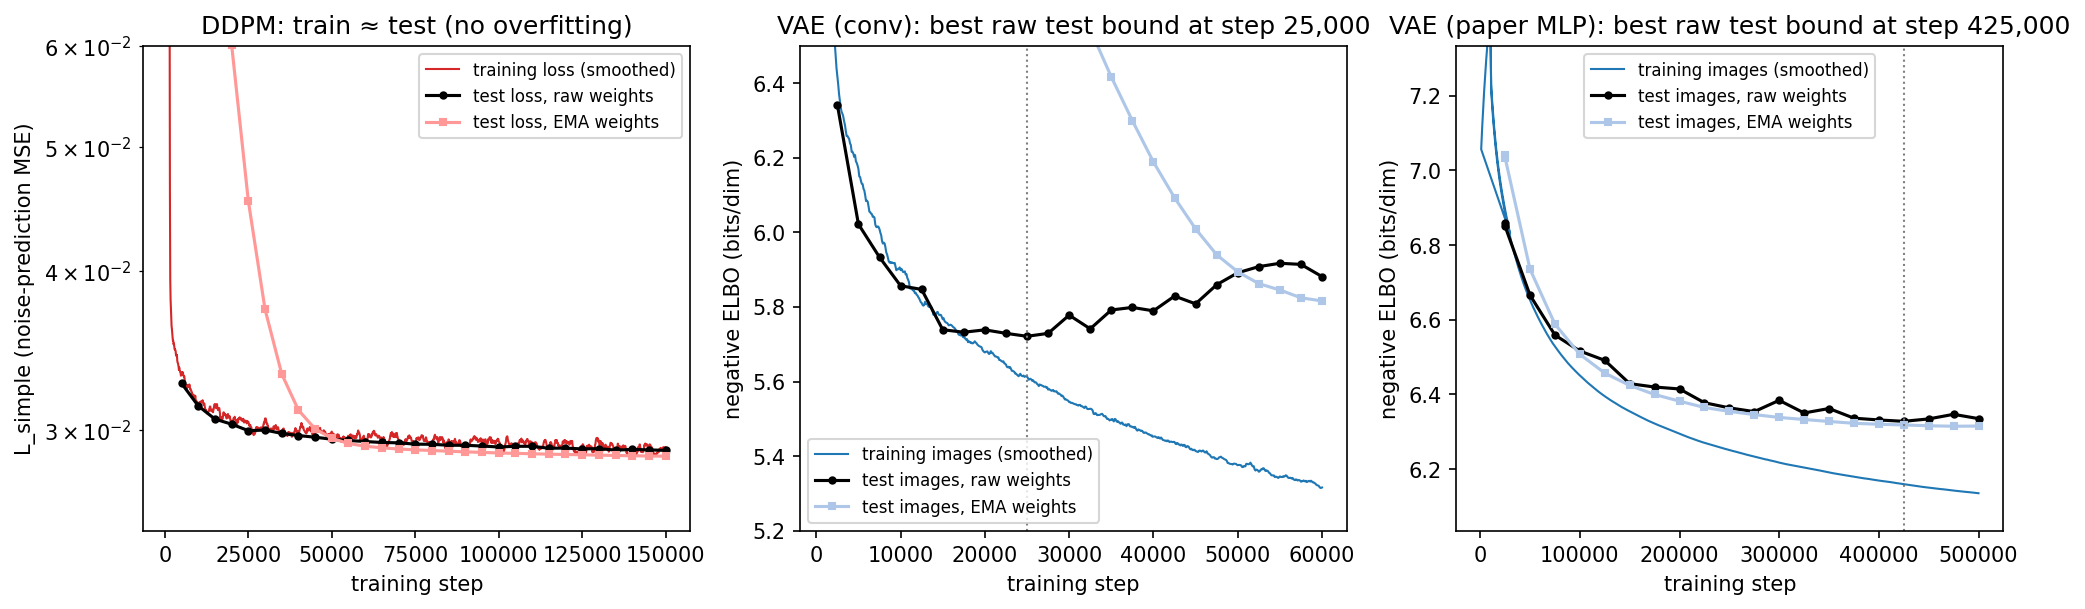
\includegraphics[width=\textwidth]{fig_training_curves.png}
\caption{Training and test objectives. DDPM: training and test losses coincide, so there is no overfitting.
VAE-Conv: the test bound is best at step 25k and then rises while the training bound keeps falling. VAE-MLP
overfits only slightly.}
\label{fig:curves}
\end{figure}

\begin{itemize}
  \item \textbf{VAE-Conv overfits its likelihood.} Its best test bound was $5.72$\,bits/dim at step $25$k. By
        step $60$k the training bound had fallen to $5.32$ while the raw-weight test bound had risen to $5.88$;
        the EMA weights we evaluate reach $5.82$.
  \item \textbf{VAE-MLP overfits only slightly:} $6.14$\,bits/dim on training images vs.\ $6.32$ on test images at
        the end of training.
  \item \textbf{The DDPM does not overfit.} Its final test loss ($0.0289$) matches its training loss ($0.0292$).
        Its EMA weights start far worse than the raw weights because, as in the paper, the EMA (decay $0.9999$) has
        no warm-up and still contains much of the random initialisation early on. They catch up after about 45k
        steps.
\end{itemize}

\begin{figure}[H]
\centering
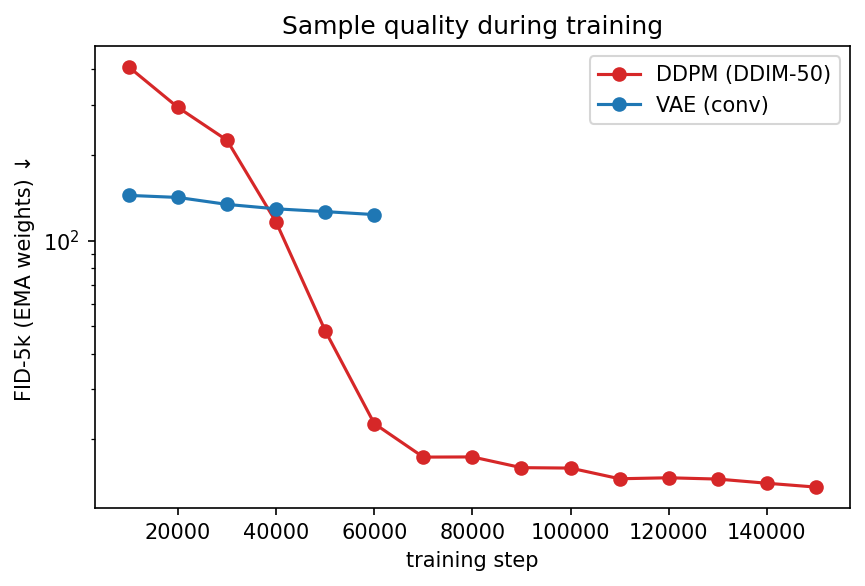
\includegraphics[width=0.62\textwidth]{fig_fid_during_training.png}
\caption{FID during training (5k samples, EMA weights; DDPM sampled with DDIM-50). The DDPM's FID keeps improving
long after its loss has flattened, and was still falling at 150k steps.}
\label{fig:fid-train}
\end{figure}

\paragraph{Likelihood and sample quality disagree.}
\begin{itemize}
  \item VAE-Conv's FID kept improving (144 $\to$ 123) while its test likelihood got worse.
  \item The DDPM's loss was flat from about 20k steps, while its FID fell from $408$ (10k steps) to $22.7$ (60k)
        and $13.6$ (150k).
\end{itemize}
This illustrates the observation of \citet{theis2016note} that likelihood and sample quality are distinct
objectives.

\paragraph{The prior hole, measured.}
\begin{itemize}
  \item VAE-Conv's \emph{reconstructions} of test images reach FID $57.9$ and recall $0.32$.
  \item Its \emph{samples} from $p(\z)$ reach FID $121.9$ and recall $0.07$.
\end{itemize}
The decoder can produce far better images than it does when sampling from the prior. The reason is that the
aggregate posterior $q_\phi(\z)=\E_{\x}\,q_\phi(\z\mid\x)$ does not fill $\N(\mathbf{0},\I)$, so a random
$\z\sim\N(\mathbf{0},\I)$ often lands where the decoder never received training signal. This is not posterior
collapse: all $128$ latent dimensions are active~\citep{burda2016iwae}, with a KL of $381$\,nats. The DDPM avoids
the problem by construction: its prior term $L_T$ is $8\times10^{-6}$\,bits/dim.

\subsection{Likelihood decomposition}

\begin{figure}[H]
\centering
\begin{minipage}[c]{0.5\textwidth}
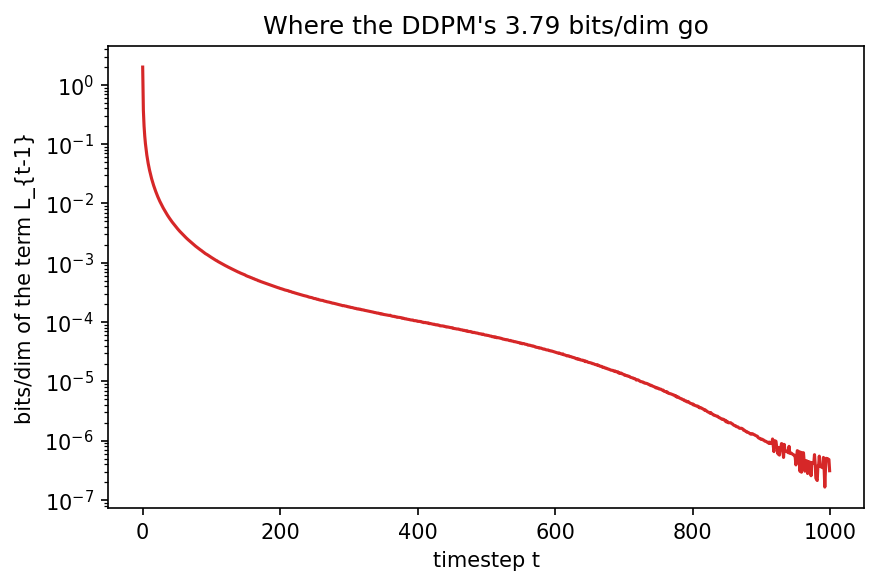
\includegraphics[width=\textwidth]{fig_bits_per_timestep.png}
\end{minipage}\hfill
\begin{minipage}[c]{0.46\textwidth}
\small
\begin{tabular}{@{}lc@{}}
\toprule
Model & Test bits/dim$\downarrow$\\
\midrule
VAE-MLP (ELBO) & $6.313\pm0.006$\\
VAE-Conv (ELBO) & $5.826\pm0.007$\\
DDPM, $\sigma_t^2=\beta_t$ & $3.794\pm0.015$\\
DDPM, $\sigma_t^2=\btil_t$ & $3.781\pm0.019$\\
\bottomrule
\end{tabular}\\[4pt]
\footnotesize $\pm$: standard error. DDPM: 1,000 test images (1000 network evaluations each); VAEs: all 10,000.
\end{minipage}
\caption{Left: contribution of each term $L_{t-1}$ of \cref{eq:vlb} to the DDPM's $3.79$\,bits/dim. Right: test
likelihood bounds of all models.}
\label{fig:bpd}
\end{figure}

Of the DDPM's $3.79$\,bits/dim:
\begin{itemize}
  \item $1.99$ ($52\%$) are spent on the final decoder term $L_0$;
  \item $3.57$ ($94\%$) are spent on the last 50 of the 1000 steps;
  \item the first $\sim\!900$ steps, where the content of the image is decided (\cref{sec:qualitative}), cost
        almost nothing.
\end{itemize}
Most of the code length therefore describes imperceptible detail, which explains how a model can have excellent
samples without a state-of-the-art likelihood. This matches the interpretation in Section~4.3 of
\citet{ho2020ddpm}. For comparison, VAE-Conv spends $0.18$\,bits/dim ($381$\,nats per image) on the KL term that
keeps its posterior close to the prior, while the DDPM's prior term $L_T$ is negligible.

\subsection{Ablations without extra training, and memorisation}

\begin{table}[H]
\centering\small
\caption{Left: effect of EMA weights (DDIM-100 for the DDPM). Right: memorisation check, i.e.\ nearest-neighbour
distance to the training set relative to unseen real test images, and the share of samples closer than the real
test images' 1st percentile (a copying model would score $\gg0.01$).}
\label{tab:ablations}
\begin{minipage}[t]{0.55\textwidth}
\centering
\begin{tabular}{@{}lcccc@{}}
\toprule
 & FID$\downarrow$ & IS & Prec. & Rec.\\
\midrule
DDPM, EMA & \textbf{9.63} & \textbf{8.24} & \textbf{0.639} & 0.584\\
DDPM, raw & 19.50 & 7.53 & 0.568 & \textbf{0.608}\\
VAE-Conv, EMA & 121.51 & 3.87 & 0.415 & 0.059\\
VAE-Conv, raw & \textbf{118.90} & \textbf{3.90} & 0.412 & \textbf{0.076}\\
\bottomrule
\end{tabular}
\end{minipage}\hfill
\begin{minipage}[t]{0.42\textwidth}
\centering
\begin{tabular}{@{}lcc@{}}
\toprule
 & NN ratio & $<$ 1st pct.\\
\midrule
VAE-MLP & 1.302 & 0.0000\\
VAE-Conv & 1.337 & 0.0000\\
DDPM & 1.024 & 0.0009\\
\bottomrule
\end{tabular}
\end{minipage}
\end{table}

\begin{itemize}
  \item \textbf{EMA halves the DDPM's FID.} For VAE-Conv it slightly \emph{hurts} FID, by more than the evaluation
        noise, although it gives the better test likelihood. This is one more instance of likelihood and sample
        quality disagreeing.
  \item \textbf{No memorisation.} DDPM samples are about as close to the training set as unseen real images are,
        and only $0.09\%$ are unusually close. \Cref{fig:nn} shows the DDPM's eight closest samples: they share pose
        and subject with their nearest training images but differ in colour, background and detail. The VAE's
        samples are far from every training image because they are blurry.
\end{itemize}

\begin{figure}[H]
\centering
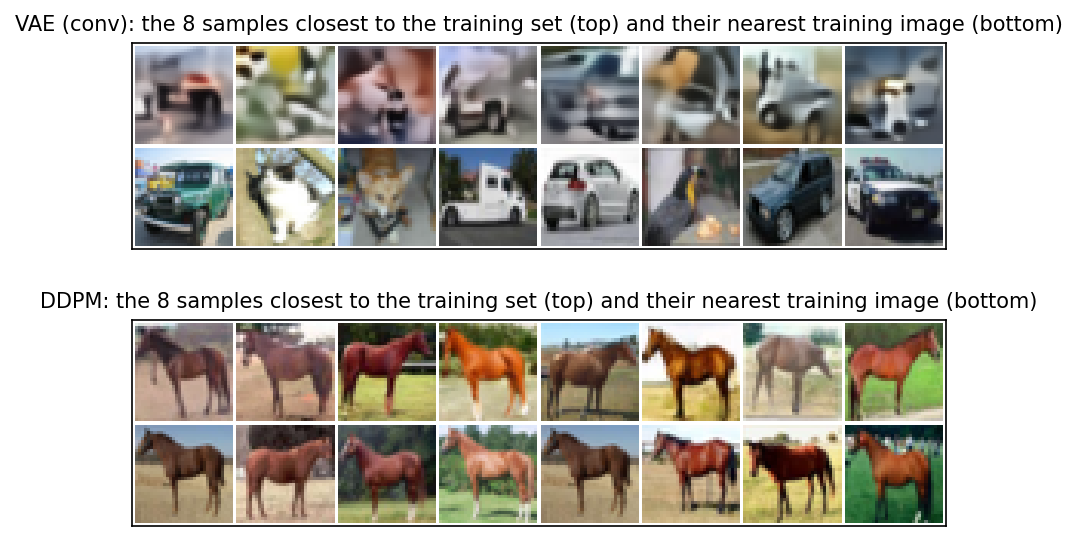
\includegraphics[width=0.8\textwidth]{fig_nearest_neighbours.png}
\caption{The eight samples closest to the training set (top row of each pair) and their nearest training images
(bottom row), in Inception feature space. Even the closest DDPM samples are new images, not copies.}
\label{fig:nn}
\end{figure}

\section{Qualitative Analysis}
\label{sec:qualitative}

All grids are \textbf{uncurated}: they show the first samples of a fixed random seed.

\begin{figure}[H]
\centering
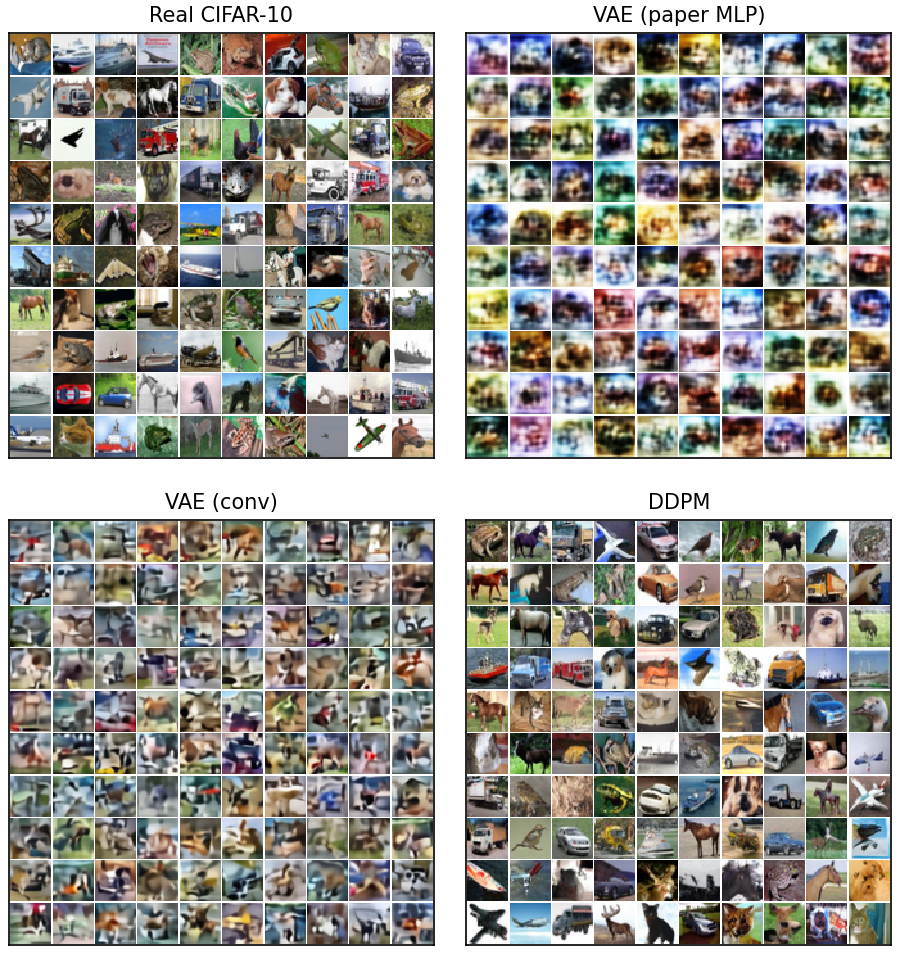
\includegraphics[width=0.86\textwidth]{fig_samples_grid.png}
\caption{Uncurated samples (first 100 of a fixed seed) of each model next to real CIFAR-10 test images.}
\label{fig:samples}
\end{figure}

\subsection{Realism}
\begin{itemize}
  \item \textbf{DDPM.} Most samples are sharp, coherent photographs with recognisable objects (horses, cars,
        trucks, ships, birds, frogs), plausible lighting and backgrounds, and correct global structure. Failures
        occur at the level of objects (implausible shapes, objects blending into the background, ambiguous
        species), while low-level texture is almost always realistic.
  \item \textbf{VAE-Conv.} Samples have plausible colours and rough layouts, typically a foreground blob on a
        background, but no sharp edges or texture.
  \item \textbf{VAE-MLP.} Samples are blurrier still: high-contrast colour blobs with little object structure.
\end{itemize}
The mechanism follows from \cref{eq:vae-recon}. The decoder models pixels as independent Gaussians, so when many
sharp images are compatible with one latent, the optimal mean is their \emph{average}, which is blurry. Each
reverse step of the DDPM, in contrast, only removes a small amount of noise. That is a nearly Gaussian problem
which a Gaussian transition models accurately, so detail survives.

\begin{figure}[H]
\centering
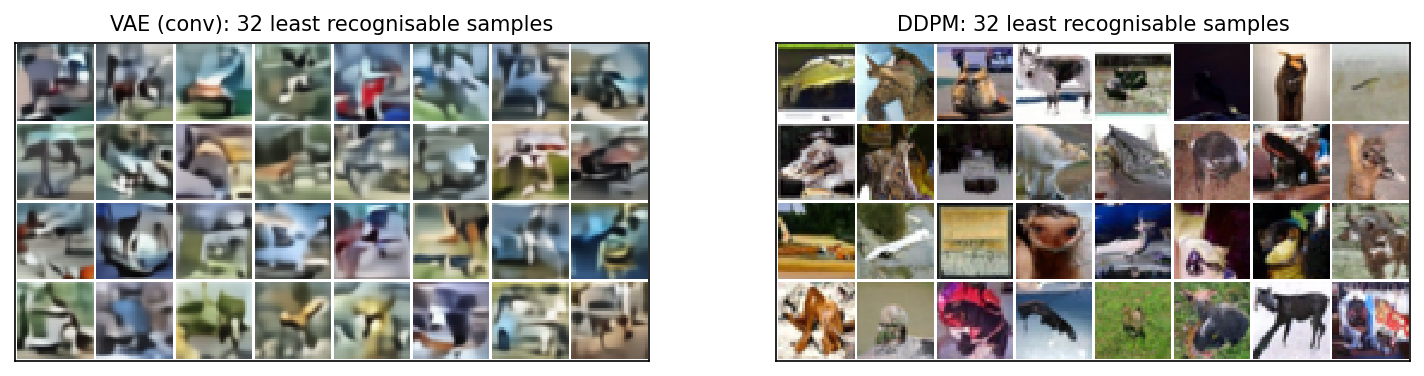
\includegraphics[width=\textwidth]{fig_failures.png}
\caption{The 32 least recognisable samples according to the classifier. The VAE's worst samples are abstract and
blurry. The DDPM's worst samples are still sharp, photograph-like images whose \emph{content} is ambiguous, as in
many real CIFAR-10 images.}
\label{fig:failures}
\end{figure}

\subsection{Diversity and thematic consistency}
The DDPM grid varies in class, colour, background, scale and viewpoint about as much as the real grid does
(recall $0.58$ vs.\ $0.69$). The VAE grids repeat similar muted colours and centred blobs (recall $0.07$).

\begin{figure}[H]
\centering
\begin{subfigure}[t]{0.49\textwidth}\centering
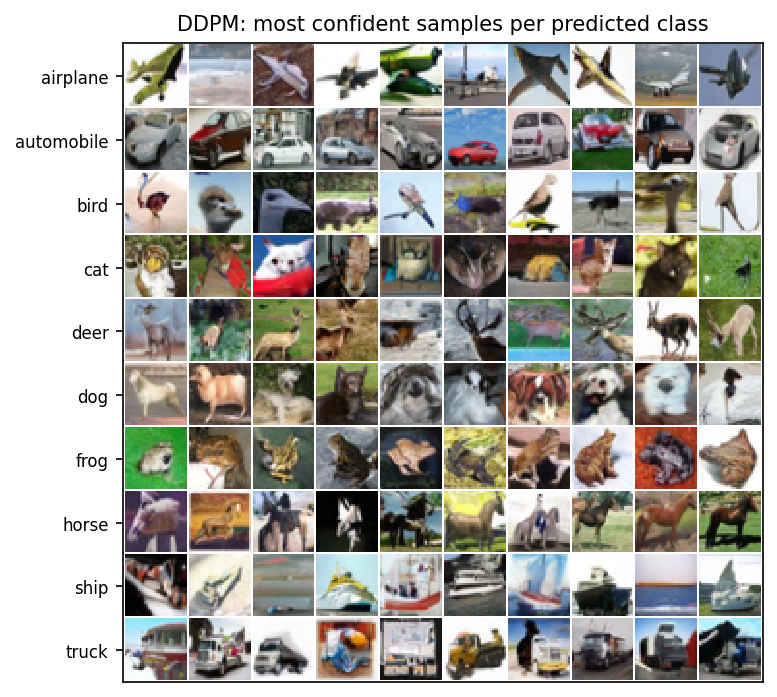
\includegraphics[width=\textwidth]{fig_by_class_ddpm_ancestral1000.png}
\caption{DDPM}
\end{subfigure}\hfill
\begin{subfigure}[t]{0.49\textwidth}\centering
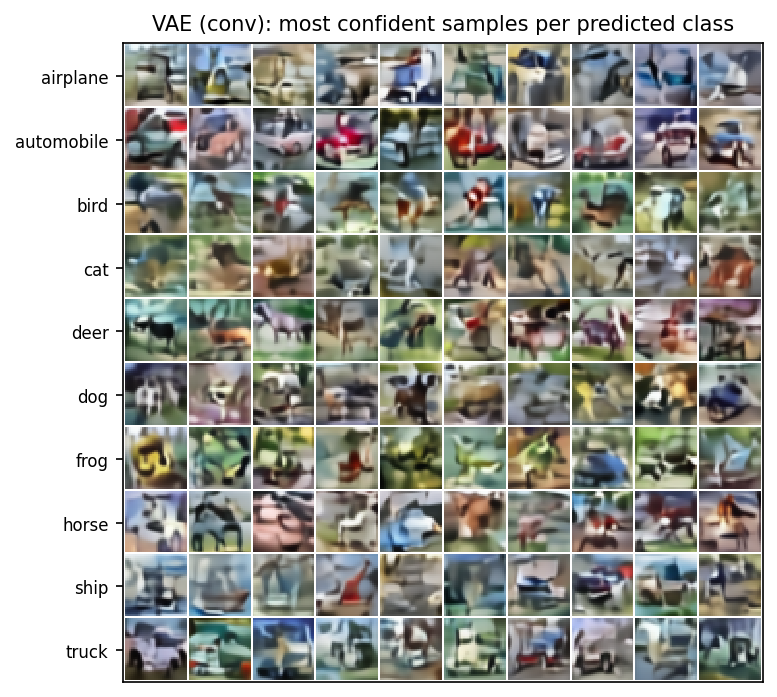
\includegraphics[width=\textwidth]{fig_by_class_vae_conv.png}
\caption{VAE-Conv}
\end{subfigure}
\caption{The classifier's most confident samples for each predicted class. DDPM samples are clear instances of
their class; even the VAE's most confident samples are only loosely related to theirs.}
\label{fig:byclass}
\end{figure}

\subsection{How each model generates}

\begin{figure}[H]
\centering
\begin{minipage}[c]{0.56\textwidth}
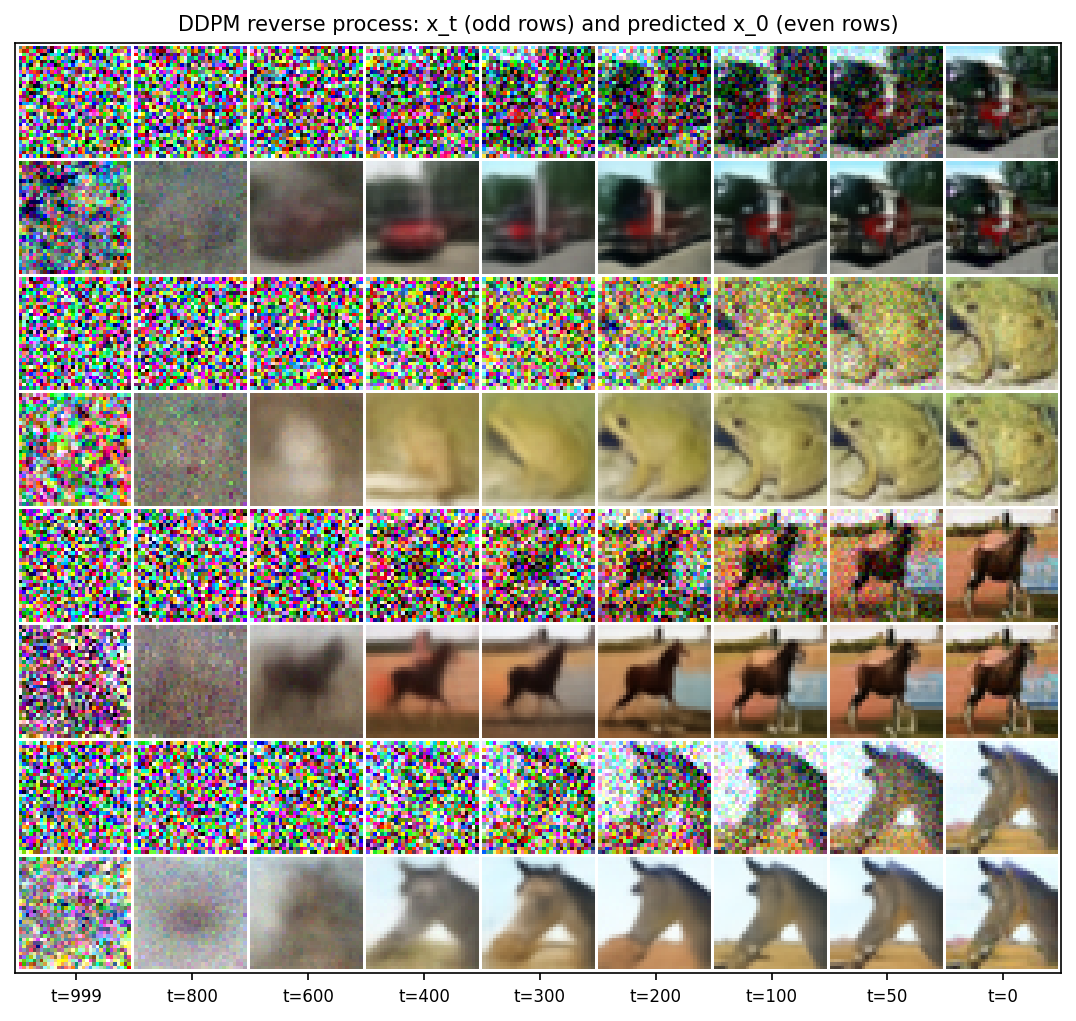
\includegraphics[width=\textwidth]{fig_ddpm_denoising.png}
\end{minipage}\hfill
\begin{minipage}[c]{0.42\textwidth}
\caption{The DDPM reverse process. Odd rows show $\x_t$ and even rows the predicted clean image $\hat\x_0$.
Generation is \emph{coarse-to-fine}: layout and colours are fixed by $t\approx600$--$400$ (a red truck, a frog, a
horse), and later steps only add detail. Together with \cref{fig:bpd}, this shows that the content is decided
early and cheaply, while most of the likelihood is spent on fine detail.}
\label{fig:denoise}
\end{minipage}
\end{figure}

\begin{figure}[H]
\centering
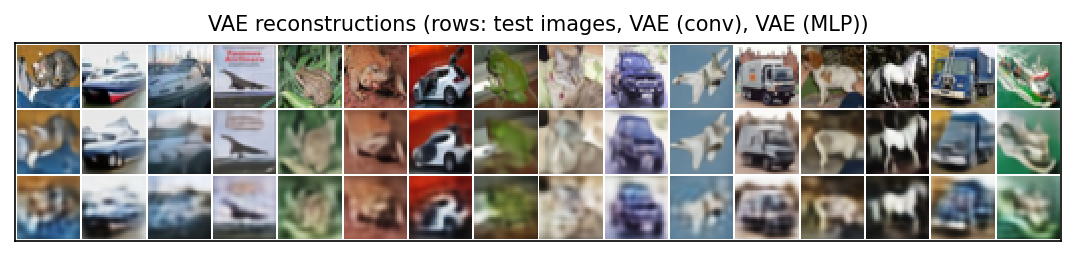
\includegraphics[width=\textwidth]{fig_vae_reconstructions.png}
\caption{VAE reconstructions. Rows: test images, VAE-Conv, VAE-MLP. Layout and colour survive the 128-d
bottleneck; texture does not.}
\label{fig:recon}
\end{figure}

The two VAEs reach almost the same PSNR ($24.07$ vs.\ $23.61$\,dB) and SSIM ($0.772$ vs.\ $0.771$) on test
reconstructions. Yet VAE-MLP's reconstructions are visibly blurrier, and their FID is far worse ($99.4$ vs.\
$57.9$). Pixel-wise metrics do not capture perceptual quality.

\subsection{Latent spaces}

\begin{figure}[H]
\centering
\begin{minipage}[c]{0.56\textwidth}
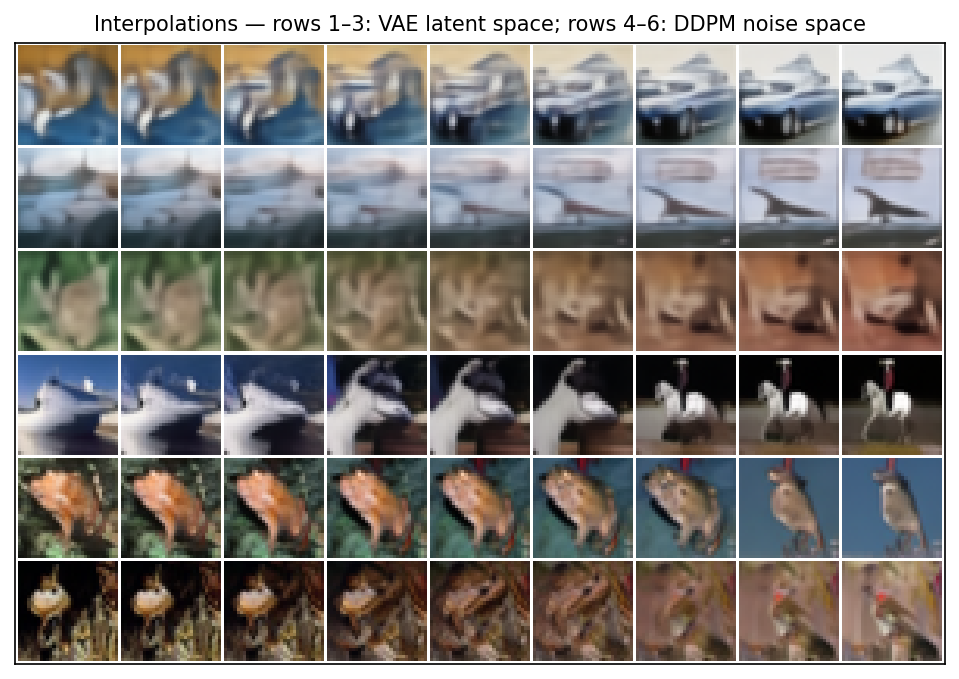
\includegraphics[width=\textwidth]{fig_interpolation.png}
\end{minipage}\hfill
\begin{minipage}[c]{0.42\textwidth}
\caption{Interpolations. Rows 1--3: linear interpolation between the VAE latents of two test images gives smooth,
gradual blends; the VAE has a learned, semantic latent space. Rows 4--6: spherical interpolation between two
DDPM starting noises $\x_T$, decoded deterministically with DDIM-50, gives sharp images throughout. The content,
however, \emph{switches} between objects rather than blending, because the DDPM's ``latent'' is simply noise.}
\label{fig:interp}
\end{minipage}
\end{figure}

\begin{figure}[H]
\centering
\begin{minipage}[c]{0.36\textwidth}
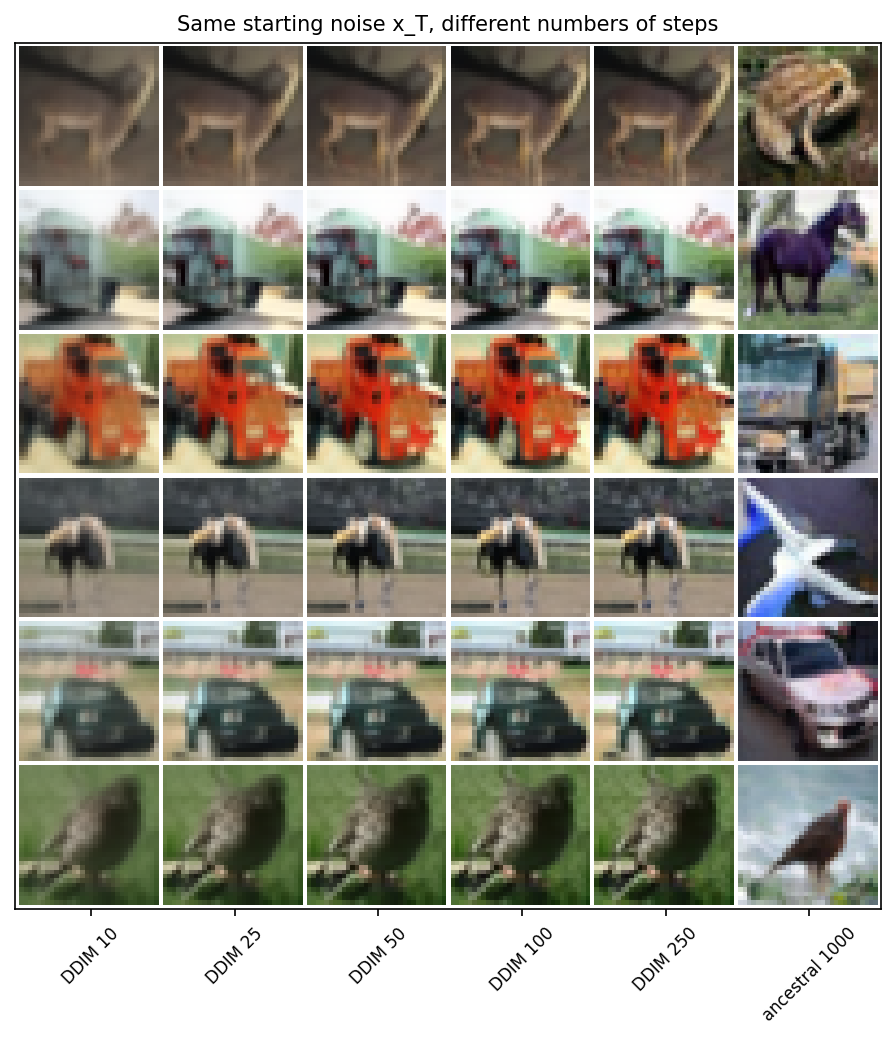
\includegraphics[width=\textwidth]{fig_ddim_steps.png}
\end{minipage}\hfill
\begin{minipage}[c]{0.6\textwidth}
\caption{The same starting noise $\x_T$ decoded with 10--250 DDIM steps, and with the 1000-step ancestral sampler
(last column). DDIM is deterministic, so every step count gives the \emph{same} image and extra steps only sharpen
details. The ancestral sampler adds fresh noise at every step, so its image differs. This is expected, not a bug.}
\label{fig:ddimsteps}
\end{minipage}
\end{figure}

\subsection{Blind rating by a vision-language model}
\label{sec:blind}

As an independent, subjective judgement, we ran a blind rating of 150 shuffled images: 50 real CIFAR-10 test
images, 50 VAE-Conv samples and 50 DDPM samples (1000-step sampler), drawn at random from the evaluated sample
sets. The rater was \textbf{Gemini}, a vision-language model, not a person. For every image it gave:
\begin{itemize}
  \item a realism score from 1 to 5;
  \item the CIFAR-10 class, or ``unrecognisable'';
  \item a verdict of real or generated.
\end{itemize}
The instructions named neither the models nor the proportions of each source, and stated that low resolution
alone is no sign of being generated.

\begin{table}[H]
\centering\small
\caption{Blind rating by Gemini (50 images per source; 95\% Wilson intervals in brackets).}
\label{tab:blind}
\begin{tabular}{@{}lcccc@{}}
\toprule
Source & Mean realism (1--5) & Named a class & Judged ``real'' & Correct class\\
\midrule
Real test images & \textbf{4.58} & 100\% & 96\% [87, 99] & 96\%\\
DDPM & 4.28 & 98\% & \textbf{96\% [87, 99]} & --\\
VAE-Conv & 1.34 & 24\% & 0\% [0, 7] & --\\
\bottomrule
\end{tabular}
\end{table}

\begin{itemize}
  \item \textbf{Gemini could not tell DDPM samples from real photographs.} It judged 48 of 50 in each group to be
        real, so its real-vs-DDPM accuracy is $50\%$, i.e.\ chance.
  \item \textbf{Its graded scores still detect a small gap.} Realism averaged $4.28$ for DDPM vs.\ $4.58$ for real
        photos (Mann--Whitney $p=0.015$), consistent with the remaining FID gap.
        DDPM samples also received fewer top scores of 5 (20 vs.\ 33 of 50).
  \item \textbf{Every VAE sample was identified as generated.} 33 of the 50 VAE samples received the lowest
        realism score, and only $24\%$ could be assigned any class, independently confirming \cref{tab:thematic}.
  \item \textbf{Almost all DDPM samples were recognisable} ($98\%$ were assigned a class), and Gemini's labels cover
        all ten classes.
\end{itemize}

\paragraph{Integrity.} All 50 ``real'' images are exact CIFAR-10 test images with the labels in the answer key, and
none of the 100 generated images appears in the test set. The rater's answers contradict the key exactly where a
blind rater would err: it labelled 48 of 50 DDPM samples ``real''. We report this single automated rater as
supporting evidence, not as a substitute for a human study.

\section{Discussion: the Main Differences between the Three Models}
\label{sec:discussion}

\subsection{VAE-MLP vs.\ VAE-Conv: the effect of the network}
The two VAEs share the method and differ only in the network (\cref{tab:arch-compare}).

\paragraph{What the convolutional network improves.}
\begin{itemize}
  \item \textbf{Likelihood:} $5.83$ vs.\ $6.31$\,bits/dim, i.e.\ a $0.49$\,bits/dim better bound.
  \item \textbf{Sample quality:} FID $121.9$ vs.\ $136.0$, and IS $3.88$ vs.\ $3.11$.
  \item \textbf{Coverage:} recall $0.073$ vs.\ $0.003$.
  \item \textbf{Reconstructions:} FID $57.9$ vs.\ $99.4$.
\end{itemize}
Convolutions share filters across positions, and attention relates distant positions. Both give the model the
spatial inductive bias that the MLP, which treats an image as 3072 unrelated numbers, lacks.

\paragraph{What it does not change.} Both VAEs remain in the same regime: blurry, low-recall samples, a large gap
between reconstructions and samples, and a collapsed class distribution. \textbf{A better network improves a VAE
but does not remove its characteristic failure modes.} The paper's own network is not the cause of the VAE's
weaknesses on CIFAR-10. It only makes them worse.

\subsection{VAE-Conv vs.\ DDPM: the effect of the generative approach}
These two models share building blocks, widths, data and optimisation settings (\cref{tab:arch-compare,tab:hparams}),
and their sizes are comparable ($30.4$M vs.\ $35.7$M parameters). Their difference is therefore attributable to
the approach. Following \cref{sec:bg-unify}, three structural differences explain all the measurements:
\begin{enumerate}
  \item \textbf{One factorised step vs.\ many small steps.} The VAE must model the whole image distribution with a
        single Gaussian with independent pixels, which forces blurry averages. That gives low precision, low IS,
        and a realism score of $1.34$ in the blind rating. Each DDPM step only has to model a small denoising
        update, for which a Gaussian is accurate. That gives precision equal to real data, and samples a
        vision-language model cannot tell from real photographs.
  \item \textbf{Learned compressive encoder vs.\ fixed non-compressive encoder.} The VAE's encoder must squeeze the
        image into $128$ numbers and match $\N(\mathbf{0},\I)$ while doing so. It never matches the prior perfectly,
        and that prior hole shows as samples far worse than reconstructions (FID $121.9$ vs.\ $57.9$), collapsed
        recall, and samples that fall between classes. The DDPM's forward process matches its prior by
        construction ($L_T\approx8\times10^{-6}$\,bits/dim) and compresses nothing.
  \item \textbf{Cost of generation.} Both advantages of the DDPM are paid for at sampling time: $1000$ network
        evaluations instead of $1$, so about $1{,}700\times$ slower. DDIM cuts this by up to $100\times$ with no
        retraining, but even 10 steps remain $17\times$ slower than the VAE.
\end{enumerate}

\subsection{Summary}

\begin{table}[H]
\centering\small
\caption{The three models at a glance (best per row in bold).}
\label{tab:summary}
\begin{tabularx}{\textwidth}{@{}l>{\raggedright\arraybackslash}X>{\raggedright\arraybackslash}X>{\raggedright\arraybackslash}X@{}}
\toprule
 & \textbf{VAE-MLP} & \textbf{VAE-Conv} & \textbf{DDPM}\\
\midrule
Sample quality (FID / IS) & 136.0 / 3.11 & 121.9 / 3.88 & \textbf{6.58 / 8.59}\\
Realism / diversity (prec. / rec.) & 0.32 / 0.003 & 0.40 / 0.07 & \textbf{0.69 / 0.58}\\
Likelihood (bits/dim) & 6.31 & 5.83 & \textbf{3.79}\\
Sampling speed (img/s) & \textbf{350{,}102} & 7{,}017 & 4.2 (DDIM-10: 416)\\
Training time (GPU-h) & \textbf{0.44} & 1.32 & 3.94\\
Learned encoder / latent code & yes, 200-d & yes, 128-d & no (latent = noise)\\
Typical failure & blurry colour blobs & blurry, between-class blobs & odd object shapes, sharp texture\\
Best use & teaching baseline & fast sampling, representation learning, compression & high-fidelity generation\\
\bottomrule
\end{tabularx}
\end{table}

\paragraph{Which model to use?} It depends on the requirement:
\begin{itemize}
  \item \textbf{Sample quality, diversity, class coverage or likelihood:} the DDPM is decisively better.
  \item \textbf{Real-time generation, or an encoder for compression or editing:} only the VAE provides these.
\end{itemize}
Modern latent diffusion models~\citep{rombach2022ldm} combine the two: diffusion runs inside the compact latent
space of an autoencoder. Our measurements show why this pairing works. The autoencoder contributes the cheap,
compressed representation the DDPM lacks, and diffusion supplies the sample quality and prior matching the VAE
lacks.

\paragraph{Lessons about evaluation.}
\begin{itemize}
  \item Likelihood and sample quality moved in opposite directions three times: VAE overfitting, the EMA
        ablation, and the DDPM's flat loss while its FID kept falling.
  \item IS alone would hide the VAE's diversity failure, and FID alone would hide the split between realism and
        diversity; precision/recall separates the two.
  \item Far from the data, the metrics stop ranking models consistently: FID and KID disagree on the two VAEs.
\end{itemize}

\section{Limitations and Threats to Validity}
\label{sec:limitations}

\Cref{tab:limitations} lists the remaining limitations of this study, how each could affect the conclusions, and
how it is addressed. None of them changes the qualitative conclusions: the gap between the DDPM and the VAEs
exceeds every source of uncertainty by more than an order of magnitude in FID.

\begin{table}[H]
\centering\small
\caption{Remaining limitations, their effect, and how they are addressed.}
\label{tab:limitations}
\begin{tabularx}{\textwidth}{@{}>{\raggedright\arraybackslash}p{3.3cm}>{\raggedright\arraybackslash}X>{\raggedright\arraybackslash}X@{}}
\toprule
Limitation & Effect on the conclusions & How it is addressed\\
\midrule
\textbf{Shortened DDPM training} (150k of 800k steps) &
Our DDPM numbers are a \emph{lower bound} on what the implementation reaches; FID was still improving
(\cref{fig:fid-train}). It can only understate the DDPM's lead. &
Disclosed as the only deviation from the paper (\cref{tab:hparams}). The likelihood bound already matches the paper
to within $0.04$\,bits/dim. Checkpoints are resumable, so training can be continued.\\
\addlinespace
\textbf{FID with 10k samples} (papers: 50k) &
FID is biased upward at smaller $N$, so our values are not directly comparable to published FID-50k. &
The protocol is stated explicitly (\cref{sec:eval}) and applied identically to every model. KID, which is unbiased
at this $N$, gives the same ranking between VAE and DDPM. Evaluation noise is measured on three independent sample
sets.\\
\addlinespace
\textbf{Final checkpoint, not best} &
The paper reports its best FID over training, which is slightly optimistic. &
Our choice was fixed in advance and avoids selection bias.\\
\addlinespace
\textbf{One training run per model} &
The $\pm$ values cover evaluation noise, not variance across training seeds. Small differences (e.g.\ between the
two VAEs) should be read cautiously. &
Conclusions rely only on differences far larger than the measured noise.\\
\addlinespace
\textbf{Classifier-based thematic metrics} &
They depend on one classifier, which behaves unpredictably on images far from real data (\cref{tab:thematic}). &
Interpreted cautiously, and cross-checked by the blind rating.\\
\addlinespace
\textbf{Automated blind rater} &
A single vision-language model is not a human study, and the answer key was accessible to it. &
Reported as supporting evidence only. The answers contradict the key where a blind rater errs, and a human rating
tool is included in the repository.\\
\addlinespace
\textbf{Original VAE method} &
Stronger VAE variants (hierarchical VAEs, learned priors) would narrow the gap. &
Out of scope by design: the task asks for the original approaches.\\
\addlinespace
\textbf{Training not compiled} &
Our benchmark measured a $1.5\times$ faster DDPM training step with \texttt{torch.compile} ($16.1$ vs.\
$10.6$\,steps/s), which was not enabled for the reported runs. This affects the training-time figures only, not the
models or results. &
Reported honestly as measured. Compilation is one configuration flag (\texttt{train.compile}) for future runs.\\
\addlinespace
\textbf{Code availability} &
A results report is only verifiable if the code is accessible. &
All code, configurations, logs, raw evaluation outputs and a reproduction guide are public at \repo.\\
\bottomrule
\end{tabularx}
\end{table}

\section{Conclusion}
\label{sec:conclusion}

We implemented a VAE and a DDPM from scratch, verified them against their papers, and compared three models on
CIFAR-10 under one validated protocol.
\begin{enumerate}
  \item \textbf{Faithful implementations.} The DDPM matches the published likelihood bound to within
        $0.04$\,bits/dim after $19\%$ of the original training. Our metrics reproduce published reference values
        on real data.
  \item \textbf{The DDPM wins decisively on quality:}
        \begin{itemize}
          \item FID $6.58$ vs.\ $121.9$ and IS $8.59$ vs.\ $3.88$;
          \item precision at the level of real data and $8\times$ the recall;
          \item even class coverage and $3.79$ vs.\ $5.83$\,bits/dim;
          \item no memorisation;
          \item samples that a vision-language model could not distinguish from real photographs.
        \end{itemize}
  \item \textbf{The VAE wins decisively on speed and structure.} It needs one network evaluation per image (about
        $1{,}700\times$ faster) and provides an encoder with a smooth, semantic latent space, which the DDPM lacks.
  \item \textbf{The network matters, but does not change the regime.} Replacing the paper's MLP with a
        convolutional network improves every VAE metric, but leaves the VAE's blur, low diversity and prior hole
        intact.
  \item \textbf{The main difference.} The VAE learns a compressed latent space and generates in one factorised
        step, which causes blur and a prior hole. The DDPM fixes its encoder and generates through many small,
        easy denoising steps, which gives quality at a high sampling cost. DDIM reduces that cost by up to
        $100\times$ while still far outperforming the VAE.
\end{enumerate}


\bibliographystyle{unsrtnat}
\bibliography{references}

\appendix
\section{Reproducibility}
\label{app:repro}

The full pipeline is available at \repo. Every result in this report is produced by the following commands
(on Google Colab, the notebook \texttt{notebooks/colab\_runner.ipynb} runs the same steps):
\begin{verbatim}
pip install -e ".[eval]"
python scripts/train.py --config configs/vae_mlp_cifar10.yaml
python scripts/train.py --config configs/vae_conv_cifar10.yaml
python scripts/train.py --config configs/ddpm_cifar10.yaml
python scripts/train_classifier.py --out runs/classifier
python scripts/evaluate.py
python scripts/make_figures.py --model-figures
python scripts/plot_training_logs.py --runs runs \
       --out runs/eval/report/fig_training_curves.png
\end{verbatim}

\paragraph{Verification.} The repository contains 32 automated tests. They check the mathematics against
independent derivations:
\begin{itemize}
  \item the forward-process posterior against a numerical Bayes computation;
  \item exact recovery of the data by both samplers given a perfect noise predictor;
  \item normalisation of the discretised likelihood;
  \item the analytic KL term against a Monte-Carlo estimate;
  \item the ELBO's loss scaling ($\beta=1$);
  \item bit-exact resumption of interrupted training runs;
  \item detection of mode collapse by precision/recall.
\end{itemize}
A further test checks that the Colab notebook contains exactly the repository's code. The executed notebook,
including all training and evaluation logs, is part of the repository.

\begin{table}[H]
\centering\small
\caption{Compute used (one NVIDIA A100-SXM4-80GB).}
\begin{tabular}{@{}lr@{}}
\toprule
Run & GPU-hours\\
\midrule
VAE-MLP, 500k steps & 0.44\\
VAE-Conv, 60k steps & 1.32\\
DDPM, 150k steps & 3.94\\
Classifier (evaluation instrument), 30 epochs & 0.02\\
\midrule
\textbf{Training total} & \textbf{5.72}\\
\bottomrule
\end{tabular}
\end{table}


\end{document}
